\documentclass{article}
\usepackage{iclr2026_conference,times}
\input{math_commands.tex}

\usepackage{amsmath,amssymb}
\usepackage{booktabs}
\usepackage{array}
\usepackage{graphicx}
\usepackage{microtype}
\usepackage{xcolor}
\usepackage{placeins}
\usepackage{float}
\usepackage{longtable}
\usepackage{url}
\usepackage{hyperref}
\hypersetup{hidelinks}

\definecolor{shareblue}{RGB}{47,105,163}
\definecolor{copyorange}{RGB}{230,126,34}
\definecolor{mutegrey}{RGB}{90,90,90}
\newcommand{\qcomem}{\textsc{Q-CoMem}}
\newcommand{\method}{\textsc{ForkAudit}}
\newcommand{\materialize}{\textsc{Source+Materialize}}
\newcommand{\share}{\textsc{Shared-Document}}
\newcommand{\mib}{\,\mathrm{MiB}}
\newcommand{\gib}{\,\mathrm{GiB}}

\title{Q-CoMem: Quantized Split Replay for Memory-Constrained Hybrid LLMs}

\author{Anonymous authors}

% Anonymous ICLR submission: keep \iclrfinalcopy commented out.
% \iclrfinalcopy

\begin{document}
\raggedbottom
\maketitle

\begin{abstract}
Repeated queries over stable documents create a capacity problem for
memory-constrained inference: exact prefix caching minimizes warm latency but
retains state across all layers, whereas dense recomputation retains nothing
but repeatedly processes the document.  We present \qcomem{}, a capacity-first
extension of CoMem split replay for hybrid LLMs.  An offline Write runs the
document through a split depth, then group-quantizes the boundary residual
together with the lower-layer KV, convolution, and recurrent state required for
later queries.  Online Read dequantizes and forks that document state, keeps
mutable request state private, replays the query through the lower layers, and
reconstructs the suffix.  A fail-closed \method{} trace validates immutability,
copy-on-write, recurrent rebinding, and call provenance because output equality
alone can miss state aliasing.

On an archival 60-item Qasper/2WikiMQA validation cohort with
Qwen3.5-35B-A3B and H20-3e, a frozen Q4/Q4/Q8 policy reduces mean retained
tensor payload from $136.235$ to $9.661$ MiB/document ($14.10\times$ smaller).
Its mean F1 (0--100) is $54.24$ versus $54.62$ for split Q16, a paired difference of
$-0.39$ points with a 95\% bootstrap interval of $[-2.04,1.08]$; this is a
selected trade-off point among the evaluated split-replay policies, not a
statistical-equivalence claim.  A separate systems execution on the eight-item
indices-6--9 subset records TTFT: full-prefix Q16 is faster
($0.163$ versus about $0.673$ s) and has higher generated-token throughput
($13.38$ versus $7.15$--$7.19$ tokens/s), while \qcomem{} TPOT is within $2.5\%$
of its $54.11$ ms value.  Thus the supported contribution is
capacity reduction with an explicit online cost, not TTFT acceleration.
Separately, shared-document KV lowers the post-priming allocated delta from
$4.901$ to $2.229\gib$ at $N=32$, and a fail-closed ownership audit exposes a
historical alias invisible to output equality.  We do not claim lower total
process memory, measured recall, edge-device performance, or broad quality
preservation.
\end{abstract}

\section{Introduction}
\label{sec:intro}

Repeated queries over stable documents are common in document QA, agents, tree
search, and best-of-$N$ decoding.  Reusing a document prefix avoids repeated
prefill, but exact caching retains per-document state at every model layer.  On
a memory-constrained deployment, that state competes with model weights,
request workspace, and other resident documents.  The resulting question is
therefore capacity-first: how much reusable document state must remain resident
for later queries, and what latency and quality costs buy a smaller footprint?

Dense recomputation and exact prefix caching form two endpoints.  The former
stores no document state but repeatedly processes the prefix; the latter gives
low warm TTFT but retains the complete prefix cache.  CoMem instead writes a
document to an intermediate depth and reuses the resulting per-token
residual~\citep{liu2026comem,liu2026understanding}.  Hybrid LLMs make this
trade-off harder: lower full-attention layers also need KV, lower linear layers
need convolution and recurrent state, and those mutable states cannot be shared
blindly across requests~\citep{yang2025gateddeltanet,lieber2025jamba}.

We introduce \qcomem{}, a quantized hybrid split-replay design.  Its offline
Write persists the split residual and all lower-layer state needed to replay a
future query, using state-type-aware low-bit packing.  Its online Read
dequantizes one document entry, shares only immutable document tensors, creates
request-local mutable state, and reconstructs the upper suffix.  This saves
retained bytes by spending suffix computation; it is not intended to dominate
exact caching on TTFT.  Because equal outputs can still hide a mutable-state
alias, we pair the design with \method{}, a phase-aware ownership trace that
checks immutability, copy-on-write (COW), recurrent rebinding, and selected call
provenance.

Our contributions follow this memory--latency--quality logic:
\begin{itemize}
  \setlength{\itemsep}{1pt}
  \setlength{\parskip}{0pt}
  \item \textbf{Complete quantized hybrid split state.}  \qcomem{} stores the
  depth-$j$ residual together with the necessary lower full-attention KV and
  lower convolution/recurrent state.  Real groupwise Q4/Q8 packing and a
  state-type/per-layer bit assignment reduce the whole retained entry rather
  than counting the residual alone.
  \item \textbf{Capacity--latency--quality measurement.}  On 60 archived
  Qasper/2WikiMQA validation items, the frozen Q4/Q4/Q8 point is
  $14.10\times$ smaller than full-prefix Q16 and changes mean F1 by $-0.39$
  points relative to split Q16.  A separate registered systems execution on
  the eight-item indices-6--9 subset reports TTFT, TPOT, and generated-token
  throughput with the adverse TTFT
  trade-off visible.  Both tables keep retained payload separate from allocator
  and process memory, and leave unmeasured Recall cells blank.
  \item \textbf{Ownership-safe reuse.}  The seven-target \method{} contract
  couples semantic relations to phase-indexed storage evidence across 96
  ownership configurations.  A historical alias corrupts the persistent base
  while output and terminal request state remain exact; the repaired path is
  storage-clean in 8/8 cells.  At $N=32$, shared-document KV separately reduces
  the post-priming allocator delta by $54.5\%$ relative to full-copy KV.
\end{itemize}

The quality and latency evidence shares the reported Qwen3.5/PyTorch/
Transformers/H20 stack.  The timing execution uses indices 6--9 from each
dataset, hence an eight-item subset of the 60-item quality cohort, under a
distinct protocol; the
larger ownership study uses fixed sequential schedules.  ``Store'' is retained
tensor payload, not total VRAM, process memory, or admitted serving capacity.
Section~\ref{sec:limitations} states the full boundary.

\begin{figure}[t]
  \centering
  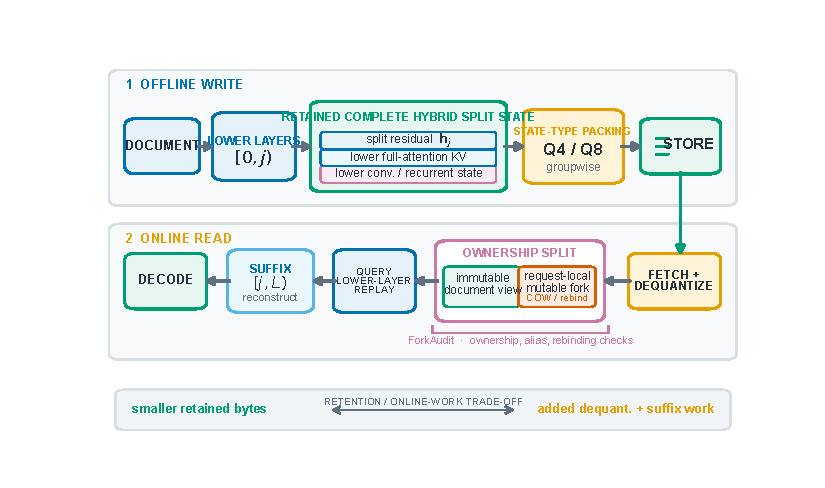
\includegraphics[width=\textwidth]{figures/qcomem_pipeline_r42.pdf}
  \caption{\qcomem{} Write/Read pipeline.  Offline Write runs the document to
  split depth $j$ and packs the complete retained state: boundary residual,
  lower full-attention KV, and lower convolution/recurrent state.  Online Read
  dequantizes the entry, shares only immutable document tensors, creates a
  request-local mutable fork through COW/rebinding, replays the query through
  the lower layers, and reconstructs the suffix.  The resulting design trades
  online work for a smaller retained document entry; \method{} checks the
  ownership boundary independently of output equality.}
  \label{fig:qcomem-pipeline}
\end{figure}

\section{Related Work}
\label{sec:related}

Prior work spans depth reuse, exact prefix caching, cache compression, hybrid
state, and relation-based testing.  \qcomem{} combines these threads around one
specific objective: reduce the complete retained state of a hybrid split-replay
entry while making request-local ownership auditable.

\paragraph{Split-depth reuse.}
CoMem persists one depth-$j$ residual per document token and executes the upper
suffix for later queries~\citep{liu2026comem,liu2026understanding}.  We build on
that interface rather than claiming a new split-replay primitive.  The added
system problem is to quantize the residual \emph{and} the lower KV/recurrent
state required by a hybrid model, then expose the capacity--latency--quality
trade-off under an explicit storage denominator.

\paragraph{Paged and prefix-aware inference.}
PagedAttention, Prompt Cache, RadixAttention, ChunkAttention, Hydragen, and
Preble establish block sharing, prefix reuse, shared-prefix computation, and
scheduling~\citep{kwon2023pagedattention,gim2024promptcache,zheng2024sglang,
ye2024chunkattention,juravsky2024hydragen,srivatsa2025preble}.  These systems
are the low-TTFT reference point; \qcomem{} deliberately trades additional
suffix work for a smaller retained document entry.

\paragraph{Hybrid state and cache management.}
Gated Delta Networks maintain mutable compact state~\citep{yang2025gateddeltanet};
Jamba, Marconi, and HYPIC address hybrid architectures or reusable hybrid
prefixes~\citep{lieber2025jamba,pan2025marconi,liu2026hypic}, while Palu,
SqueezeAttention, and HeadKV compress or budget KV~\citep{chang2025palu,
wang2025squeezeattention,fu2025headkv}.  \qcomem{} differs by jointly accounting
for the split residual and the lower hybrid state.  \method{} validates the
immutable-document/mutable-request boundary rather than replacing these cache
policies; Appendix
Table~\ref{tab:published-context} separates published numbers from our controls.

\paragraph{Evaluation and metamorphic testing.}
SCBench emphasizes cache lifecycles~\citep{li2025scbench}; metamorphic testing,
MT-DLComp, and CRADLE motivate preserved relations and independent checks
\citep{chen2018metamorphic,xiao2022metamorphic,pham2019cradle}; DNNMem separates
memory denominators~\citep{gao2020dnnmem}.  Appendix Table~\ref{tab:closest}
gives our component-wise boundary.

\section{Methodology}
\label{sec:method}
\label{sec:contract}

\subsection{Capacity-first objective and state decomposition}

Let a stable document $D$ be written once and queried repeatedly.  A deployment
must fit model weights, shared adapters, active workspace, retained document
entries, and runtime state:
\begin{equation}
 M_{\mathrm{device}} \geq M_{\mathrm{weights}}+M_{\mathrm{shared}}
 +M_{\mathrm{active}}+\sum_{D\in\mathcal{H}}S(D)+M_{\mathrm{runtime}},
\end{equation}
where $\mathcal{H}$ is the hot document set.  \qcomem{} targets $S(D)$; it does
not compress model weights or promise a smaller active workspace.  We therefore
optimize retained bytes subject to measured latency and quality, and report
allocator measurements under a separate denominator while leaving process/NVML
memory unmeasured.

For split depth $j$, the complete reusable hybrid state comprises the document
boundary residual $h_j^D$, lower-layer full-attention KV, and lower-layer
convolution/recurrent state.  With quantizer $Q_b$, its retained payload is
\begin{equation}
 S_{\mathrm{QCoMem}}(D;j,\mathbf b)=|Q_{b_h}(h_j^D)|+
 \sum_{\ell<j,\ell\in\mathcal A}|Q_{b_\ell}(K^D_\ell,V^D_\ell)|+
 \sum_{\ell<j,\ell\in\mathcal G}|Q_{b_\ell}(C^D_\ell,G^D_\ell)|.
\end{equation}
Counting only $h_j^D$ would understate the deployed state, especially for a
hybrid architecture.

\subsection{Quantized hybrid split replay}

\paragraph{Offline Write.}
The document runs through layers $[0,j)$.  We retain $h_j^D$ and the lower
attention and recurrent cache leaves needed to process a later query.  Each
floating tensor is partitioned into groups of 64 values.  For a $b$-bit group
with minimum $m$ and maximum $u$, we store
\begin{equation}
 s=(u-m)/(2^b-1),\qquad q=\operatorname{clip}
 \bigl(\operatorname{round}((x-m)/s),0,2^b-1\bigr),
\end{equation}
with packed unsigned values and BF16 scale/bias metadata.  Q16 is the BF16
unpacked reference.  State types may use different widths; the evaluated
Q4/Q4/Q8 point assigns Q4 to the residual and lower full-attention state and Q8
to lower linear state.  The reported per-layer policy uses a Q4 residual, Q16
projections, and active-layer widths $[8,8,4,4,8,8,8]$ selected on a disjoint
four-item calibration set.  We treat it as one frozen operating point, not as a
general claim that layer-wise selection is optimal.

\paragraph{Online Read.}
For each query, the packed entry is dequantized into a logical document view.
Immutable document tensors may be shared, whereas cache leaves that kernels can
mutate are cloned or rebound into request-local storage.  Query tokens traverse
the lower layers using this state; document and query residual chunks then seed
the suffix, which is executed through layers $[j,L)$ before incremental greedy
decoding.  Keeping the document and query chunks distinct is necessary for the
Qwen3.5 hybrid recurrence.  The design thus exchanges suffix reconstruction
and dequantization for a smaller per-document retained entry.

\subsection{Ownership-safe forks and fail-closed validation}

For resident requests \(r\in\{1,\ldots,N\}\), let \(\mathcal A\) and
\(\mathcal G\) denote full-attention and recurrent layers.  A logical fork is
\begin{equation}
  \mathcal{F}_r(D)=
  \bigl(\{K^D_\ell,K^r_\ell\}_{\ell\in\mathcal A},
        \{G^D_\ell,G^r_\ell\}_{\ell\in\mathcal G}\bigr),
\end{equation}
where document state \(K^D_\ell,G^D_\ell\) is immutable and may be shared,
whereas append reservations \(K^r_\ell\) and mutable recurrent state
\(G^r_\ell\) are request-local.  A borrowed recurrent base is read-only at
setup and must rebind to private storage when the registered transition first
mutates it; a partial KV tail is copied before append.

\method{} validates this lifecycle with seven targets: frozen identity, prefix
immutability, private ownership, tail-safe COW, bounded host-side call
provenance, cross-arm semantic equivalence, and cross-\(N\) prefix consistency.
For case specification \(\Sigma\), execution trace \(\tau\), mandatory slots
\(M_i(\Sigma)\), and replay predicates \(\Phi_i\),
\begin{equation}
  \operatorname{Pass}_i(\tau)\Longleftrightarrow
  [\operatorname{Coverage}_i(\tau)=\mathrm{complete}]
  \wedge\operatorname{Bind}_{\Sigma}(\tau)
  \wedge\bigwedge_{\phi\in\Phi_i}\phi(\tau).
\end{equation}
Coverage is therefore separate from verdict: a missing, duplicated, modified,
or unbound mandatory receipt cannot silently pass.  Targets 2--5 are
pre-output storage/call obligations; targets 6--7 compare registered semantic
observables and cannot substitute for ownership evidence.

This is an offline, non-adversarial regression contract, not security
attestation.  Capture/replay, the mandatory-slot schema, correct
slot-to-live-tensor binding, and framework storage semantics form the trusted
computing base (TCB).  A pass establishes only that the registered predicates
held at captured points under that TCB; it does not cover coherent
omission/fabrication, transient writes between observations, compiled GDN,
underlying ATen/CUDA, or device/driver execution.

\subsection{Capture, replay, and sensitivity checks}

The workflow freezes code, model, data, schedule, and runtime roles; captures
setup, transition, and final digests, ranges, calls, semantics, and allocator
snapshots; then replays every applicable predicate with complete/partial/open
coverage reported separately from pass/fail/not-evaluated.  The selected-cell
hook additionally binds the actual builder, direct clone lineage, and serializer
rows at three phases, while the separate dispatch run binds the selected
host-side attention artifact/configuration immediately before invocation and
seals it after normal return.  Appendix~\ref{app:storage-schema} and
Table~\ref{tab:normative-records} give the full target-to-record matrix.

Sensitivity uses matched live mutations, designer--executor-separated controls,
a dense CPU-FP32 attention sidecar, and a candidate-import-free NumPy GDN oracle
at frozen operator boundaries.  A historical pre-fix request preserved output
and terminal request state while retaining an invalid mutable base alias; the
trace failed at transition binding and base immutability, and the repaired path
passes in 8/8 cells.  This motivates the audit component without turning the
fixed controls into a population-rate claim.
\section{Experiments}
\label{sec:experiments}
\label{sec:protocol}

\subsection{Experimental setup}

\paragraph{Quality cohort.}
The broadest Store--F1 panel is an archival, raw-first validation run on
Qwen3.5-35B-A3B, PyTorch~2.11.0+cu129, Transformers~5.14.1, and eight H20-3e
GPUs.  It contains 60 paired items: Qasper and 2WikiMQA source indices 6--35,
or 30 examples per dataset, under official LongBench-v1 prompts and a
4,096-token input cap.  Qasper permits at most 128 generated tokens and
2WikiMQA at most 32.  We compare dense recomputation, full-prefix Q16/BF16,
split-replay Q16/BF16, frozen state-type Q4/Q4/Q8, same-memory per-layer mixed
precision, and an aggressive mixed policy.  Four calibration prompts (indices
4--5 from each dataset) precede and are disjoint from validation.  The archived
raw shards provide retained Store, predictions, references, and LongBench
answer F1, but not timing or Recall.

\paragraph{Latency execution.}
A separate registered systems execution uses the same model family in BF16,
PyTorch~2.11.0+cu129, and Transformers~5.14.1.  Eight validation items comprise
four Qasper and four 2WikiMQA examples at source indices 6--9.  These items are
a subset of the 60-item quality cohort, not an independent replication; the
execution and aggregation protocol is separate and the two tables are not
pooled.  Each item uses one H20-3e, a 4,096-token input cap, greedy decoding, at
most 32 generated tokens, and three timing repeats per configuration.  It
compares no-cache dense recomputation,
full-prefix Q16/BF16 reuse, uniform Q8 and Q4 \qcomem{} states, state-type
Q4/Q4/Q8, and the frozen per-layer point.  Metrics are retained Store per
document, TTFT, time per output token (TPOT), generated-token throughput, and
answer F1.  Recall was not recorded.

\paragraph{Ownership-audit cohort.}

Primary feasibility uses one fixed Qwen3.5-35B-A3B configuration
\citep{qwen2026qwen35,qwen2026qwen35modelcard}: ten vLLM-0.26 Triton
full-attention layers with BF16 KV (the protocol's ``Q16'' storage label, not
quantization) and 128-token pages, plus thirty
Transformers-torch GDN layers.  Eight H20-3e ranks run one book each with
batch-one sequential calls on one CUDA stream/rank.  In the fresh formal rerun,
each registered attention call binds the selected hashed Triton kernel-cache
artifact and compile configuration before invocation and seals the receipt only
after the original launcher returns normally on the same assigned GPU and
stream.  GDN calls bind the mutually exclusive frozen eager
routes; each GDN state digest covers 60 tensors.

Each distinct PG-19 book~\citep{rae2020compressive} supplies a 4,095-token
document and 32-token registered transition.  Four cells evaluate
$N\in\{1,8,32\}$ and eight argmax outputs; the query plus seven fed-back outputs
give 39 state-appended tokens and exercise COW on the 127-token final page.
Appendix Table~\ref{tab:cohorts} separates all supporting cohorts.  A distinct
\texttt{tiiuae/Falcon-H1-0.5B-Base} track~\citep{zuo2025falconh1} freezes
Transformers 5.14.1 on H20 and the official
\texttt{DynamicCache} reference, $N\in\{1,2\}$, and persistent lossless-Q16
versus deep-materialized candidate arms.  It tests exact relational transfer
for that naive-path configuration, not performance, memory, or quality.

\subsection{Ownership-audit procedure}

Each primary-factorial cell binds identity, rebuilds allocator and witness
executions, records setup--transition--final ownership, and compares tokens,
logits, logical KV, and GDN state.  Replay adds fixed-axis projections, one
dense-FP32 sidecar per rank, and matched live faults.  A separate PDF-only
designer freeze supplies five executor-separated pairs.  Aggregation requires
every byte binding.  Appendix Table~\ref{tab:witness} states target strength.

The stronger hook wraps only the selected $N=8$
shared-document/materialized-GDN ownership witness.  Per rank,
$60=30\times2$ denotes persistent layer/family coordinates,
$480=8\times60$ direct clone destinations, and each phase contains the full
$540=(1+8)\times60$ serializer-row universe with six owner-row anchors.  The
same schedule separately enumerates $12=3\times4$ clean-memory calls per rank
(96 total).  Zero selected-context overlaps means only that this context never
entered an allocator cell, not that the wrapper was absent or perturbation-free.

\subsection{Controls, schedules, and oracles}

The primary factorial uses sequential round-major steps on one CUDA stream per
rank.  Full logits use shape/dtype-bound CPU-FP32 bytes; KV, GDN, bases, calls,
storage, and allocator records use typed digests.  Detached replay cannot
reconstruct unarchived tensors or recapture the producer.  A preregistered
NumPy oracle checks four GDN transitions at global model-layer indices
$0,10,20,38$ after native q/k normalization against four wrong recurrences.

Supporting protocols move GDN reconstruction to a spawn-created CUDA-IPC
observer and record CUDA-event-bracketed model-call intervals around cancel,
scrub, reclaim, and replacement.  Appendix Table~\ref{tab:cohorts} fixes their
geometry and authorization.

\subsection{Memory denominators}
\label{sec:denominators}

We separate logical state, pages, synchronized allocator bytes, and unmeasured
service capacity.  In both deployment tables, ``Store'' denotes retained tensor
payload, but the accounting implementations differ: the 60-item panel sums the
stored persistent components (packed residual data, scales, biases, and unique
lower-cache tensor storage), whereas the eight-item execution measures the
physical byte-range union owned by one retained entry.  Neither denominator
includes non-tensor/Python metadata, allocator pools, process/NVML memory,
active workspace, or admission capacity, and their differently aggregated
values are not pooled.

\subsection{Retained state, latency, and answer quality}

Table~\ref{tab:qcomem-validation60} reports the broadest current
retained-state--quality cohort.  Moving from full-prefix Q16 to split Q16 first
reduces mean Store from $136.235$ to $34.683$ MiB/document ($3.93\times$
smaller).  Quantizing the complete split state with the frozen Q4/Q4/Q8 policy
reduces it further to $9.661$ MiB/document: $14.10\times$ smaller than the
full-prefix reference, or a $92.91\%$ reduction.  Mean F1 is $54.24$ versus
$54.62$ for split Q16, with a paired difference of $-0.39$ points and 95\%
bootstrap interval $[-2.04,1.08]$.  No item crosses the registered
catastrophic threshold.  This is a selected trade-off point among the evaluated
split-replay policies; the interval crossing zero does not prove equivalence or
noninferiority.

The same-memory per-layer policy saves only $2.75\%$ Store relative to the
frozen state-type policy, while its mean-F1 difference is more negative and
one of 60 items crosses the catastrophic threshold.  The aggressive policy
reaches $18.08\times$ compression but its interval against split Q16 lies below
zero and five of 60 items cross that threshold.  We therefore use frozen
Q4/Q4/Q8 as the headline operating point and treat both mixed policies as
ablations, not improvements.

\begin{table}[t]
\caption{Retained-state--quality trade-off on the 60-item archival validation
cohort (30 Qasper, 30 2WikiMQA).  TTFT and Recall columns are blank because
this run recorded neither metric.}
\label{tab:qcomem-validation60}
\centering\scriptsize
\setlength{\tabcolsep}{3.1pt}
\begin{tabular}{@{}lrrrrrl@{}}
\toprule
\multicolumn{7}{@{}l}{\emph{Dataset: Qasper (30 items) + 2WikiMQA (30 items)}}\\
Retained state & Store (MiB/doc) & vs. prefix & TTFT (s) & F1 (0--100) & Recall &
$\Delta$F1 vs. full-prefix [95\% CI] \\
\midrule
No-cache dense recompute & -- & -- & & 54.29 & & $-0.39$ [$-4.66$, $2.60$] \\
Full-prefix, native dtype & 136.235 & 1.00$\times$ & & 54.68 & & $0.00$ [$0.00$, $0.00$] \\
\qcomem{} split Q16 & 34.683 & 3.93$\times$ & & 54.62 & & $-0.06$ [$-0.18$, $0.00$] \\
\qcomem{} frozen Q4/Q4/Q8 & 9.661 & 14.10$\times$ & & 54.24 & & $-0.45$ [$-2.06$, $0.99$] \\
\qcomem{} same-memory mixed & 9.395 & 14.50$\times$ & & 53.36 & & $-1.32$ [$-4.33$, $0.92$] \\
\qcomem{} aggressive mixed & 7.536 & 18.08$\times$ & & 49.19 & & $-5.50$ [$-11.58$, $-0.20$] \\
\bottomrule
\end{tabular}
\vspace{0.5mm}
\parbox{0.97\textwidth}{\scriptsize Store and F1 are 60-item means. Every column, compression included, uses one
reference arm: the full-prefix entry as the unmodified stack retains it, in its
native dtypes. $30.000$ MiB/document of that $136.235$ MiB is FP32 GDN
recurrent state in excess of a BF16 encoding; an all-BF16 reference is
$106.235$ MiB/document, giving $1.00/3.7038/10.9965/11.3073/14.0969\times$ for
the rows above. Intervals are paired 10,000-resample item-level bootstrap
percentile intervals against full-prefix (seed 20260902); deltas use unrounded
means. The catastrophic-regression count is 0/60 against dense under the
registered $\leq-50$ point rule and 0/60 against full-prefix. An interval
crossing zero is not statistical equivalence, and the headline policy was
selected on this panel without multiplicity adjustment.
Appendix~\ref{app:all-intervals} gives the method and all 42 intervals; blank
cells are unmeasured metrics, not zeros.}
\end{table}


Table~\ref{tab:qcomem-tradeoff} provides the separate timing characterization
on the eight-item indices-6--9 subset.
On these eight items, Q8 retains $15.89$ rather than $140.34$ MiB/document
($88.68\%$ less) at the same measured mean F1 of $39.137$.  The calibrated
per-layer point retains $9.74$ MiB/document ($93.06\%$ less) with a mean-F1
change of $-0.022$ points.  Uniform Q4 reaches $8.41$ MiB but loses $3.047$ F1
points, making it an aggressive-bit failure endpoint rather than the headline
operating point.

The latency result is not a speedup over exact caching.  Full-prefix Q16 records
$0.163$ s TTFT, whereas the \qcomem{} rows are approximately $0.673$--$0.674$
s because they dequantize and rebuild the suffix.  Their TPOT is within $2.5\%$
of full-prefix ($54.97$--$55.44$ versus $54.11$ ms), but median generated-token
throughput falls from $13.38$ to $7.15$--$7.19$ tokens/s; dense recomputation
has $648.75$ ms TPOT.  Thus the supported result is a retained-capacity
trade-off with explicit online cost, not universal latency improvement.

\begin{table}[t]
\caption{Capacity--latency--quality trade-off from a separate execution on the
registered eight-item Qasper/2WikiMQA slice (source indices 6--9 of each
dataset), a subset of the 60-item panel rather than an independent
replication.  All rows use Qwen3.5-35B-A3B, PyTorch~2.11.0+cu129,
Transformers~5.14.1, one H20-3e per item, a 4,096-token cap, greedy decoding,
at most 32 generated tokens, and three timing repeats.}
\label{tab:qcomem-tradeoff}
\centering\scriptsize
\setlength{\tabcolsep}{3.0pt}
\begin{tabular}{@{}lrrrrrrr@{}}
\toprule
\multicolumn{8}{@{}l}{\emph{Dataset: Qasper (4 items) + 2WikiMQA (4 items)}}\\
Retained state & Store (MiB/doc) & Reduction & TTFT (s) & TPOT (ms) & tok/s & F1 (0--100) & Recall \\
\midrule
No-cache dense recompute & 0.00 & -- & 0.649 & 648.75 & 1.36 & 39.42 & \\
Full-prefix, native dtype & 140.34 & reference & 0.163 & 54.11 & 13.38 & 39.14 & \\
\qcomem{} Q8 & 15.89 & 88.68\% & 0.673 & 55.44 & 7.15 & 39.14 & \\
\qcomem{} Q4/Q4/Q8 & 10.01 & 92.87\% & 0.674 & 54.97 & 7.19 & 39.01 & \\
\qcomem{} per-layer mixed & 9.74 & 93.06\% & 0.673 & 55.07 & 7.19 & 39.11 & \\
\qcomem{} Q4 & 8.41 & 94.01\% & 0.674 & 55.02 & 7.19 & 36.09 & \\
\bottomrule
\end{tabular}
\vspace{0.5mm}
\parbox{0.97\textwidth}{\scriptsize Store, timing, and throughput columns are medians over the eight documents,
whereas the 60-item panel reports means over a cohort with $3.8\%$ shorter
documents, which is why its full-prefix figure is $136.235$ rather than
$140.34$ MiB. Store is the byte-range union owned by one retained entry and
excludes non-tensor/Python metadata, allocator pools, process/NVML memory,
workspace, and admission capacity. The reference is the entry in the stack's
native dtypes: $42.8\%$ of its $140.34$ MiB is FP32 GDN recurrent state, so
part of every reduction is dtype narrowing rather than packing. F1 is the
eight-workload mean and this execution is not pooled with the 60-item panel.
The per-layer policy uses a Q4 residual and layer bits $[8,8,4,4,8,8,8]$ from a
disjoint four-item calibration set; its mean-F1 delta is $-0.022$, Q8's is
$0.000$. The all-Q4 row is the aggressive failure endpoint, and Recall was not
measured.}
\end{table}


\subsection{Audit controls and governance}

Pre-output ledgers bind code, model, data, queries, and protocol.  Nine matched
live mutations, a preregistered target-gate-suppression matrix, and five
designer--executor-separated constructed controls use frozen loci, predicates,
and precedence; they establish fixed-case sensitivity and localization, not a
rate.  A separate no-injection historical protocol compares fresh pre-fix,
repaired-borrowed, and materialized $N=2$ lanes for one previously observed
alias mechanism.  Appendix~\ref{app:invariants} records the detailed rows.

\subsection{Ownership and correctness results}
\label{sec:results}

\subsubsection{Primary trace validation}
\label{sec:target-status}

All seven targets have complete mandatory-trace coverage and satisfy the
registered pass criterion for the fresh frozen primary rerun.  For target 5,
host-side receipts for 209,920 attention calls record the selected hashed
Triton artifact/configuration and autotune/no-autotuner decision immediately
before the original Python launcher, then seal after normal return.  Another
635,520 receipts record the mutually exclusive GDN eager route and functional
cache rebind.  The totals factor as $20{,}992\times10$ attention calls and
$20{,}992\times30$ request-GDN calls plus $192\times30$ one-time prefill calls.
They establish host-side selected launch/configuration provenance only, not
device-side operator identity, execution, or completion, compiled GDN,
underlying ATen/CUDA, or driver/device binaries.

\subsubsection{Ownership evidence and allocator result}

Across $8\times3\times4=96$ configurations (192 rebuilt allocator/witness
cells), tokens, full logits, final logical KV, final GDN, both fixed-axis
projections, and all 288 adjacent-fan-out comparisons match exactly.  These
semantic relations are paired with physical ownership evidence: borrowed GDN
starts as 60 immutable base aliases/request, materialized setup is disjoint,
and completed requests in both setup arms rebind at the registered 32-token
transition boundary to 60 request-private tensors disjoint from bases and
completed peers.  The evaluated
ownership and immutability predicates pass at setup, transition, and final
capture; the bounded host-side receipts also pass
(Section~\ref{sec:target-status}).  The $N=1$
cells directly exercise request--base disjointness.

\paragraph{Selected-cell builder-to-receipt live binding.}
The V29 rerun is terminally complete and scientifically valid on all eight
ranks.  Its same-run selected witnesses yield
$8\times3\times6=144$ selected-owner-row checks,
$8\times3\times540=12{,}960$ full serializer/live-object rows,
$8\times480=3{,}840$ direct clone edges, and $8\times3=24$ stable artifacts.
All 96 separately enumerated clean-memory calls occur outside the active
selected context.  Other cells and the honest-process assumption remain
outside this stronger binding.

\paragraph{Allocator reduction with canonical equality.}
With materialized GDN setup at $N=32$, switching from full-copy to
shared-document KV reduces final allocated delta from $4.901$ to $2.229\gib$,
a $54.5\%$ reduction above the frozen post-priming baseline, while the
registered observables are canonically equal across the compared ownership
arms.  Borrowed GDN changes allocation timing
rather than the shared-KV end state: its corresponding full-copy and
shared-document endpoints are $4.890$ and $2.229\gib$, and both shared-document
cells finish at $2.229\gib$.  Appendix Table~\ref{tab:rr2-memory} reports all
four endpoints under the distinct allocator denominator.

\paragraph{Falsification beyond output equality.}
All 44 clean captured-boundary numerical rows pass and all 44 seeded
wrong-operator controls are rejected.  Nine matched controls and five
designer--executor-separated controls also pass, while every paired mutant is
rejected at its frozen gate; token equality catches $0/5$ of the semantic-complete
mutants and exact logits catch $1/5$.  In the historical case, output and
terminal request state remain exact in 8/8 cells despite persistent-base
corruption, whereas the repaired path is storage-clean in 8/8.  Appendix
Tables~\ref{tab:rr2-mutants}--\ref{tab:r35-historical-alias} give the fixed-case
rows and captured-boundary qualifications.

Supporting cohorts extend the lifecycle through cancellation/reclamation,
derive 1,080 GDN observations and 96,660 relations from a source-distinct
expected-slot census, and reproduce them in a second execution.  A separate
Falcon-H1 configuration matches its official Transformers reference on all
registered token, logit, state, and ownership checks.  These bounded checks do
not supply additional \qcomem{} performance or quality evidence; protocol and
transfer details remain in the appendix.

\subsection{Limitations and scope}
\label{sec:limitations}

The quality panel contains 60 Qasper/2WikiMQA validation items on one
Qwen3.5/H20 stack; the latency panel is a separate execution on its eight-item
indices-6--9 subset, not an independent replication.  The tables are not
pooled.  They support the stated bounded point estimates, not broad benchmark
quality preservation.  The
60-item run is archival raw-first evidence: hashes, raw predictions, F1,
bootstrap intervals, and Store accounting replay, but the original launcher
used a mutable code directory and retained neither a pre-run full-source ledger
nor a full model-weight ledger.  We therefore do not describe it as fresh
source-frozen regeneration.  The 60-item run has no timing measurements; neither
cohort measured Recall, whose table cells remain blank.

H20 is not an edge device; memory-constrained local or edge use is the
motivation, not an evaluated hardware claim.  The calibrated per-layer row is
one operating point selected from four disjoint items, and the current
implementation has substantially higher TTFT than full-prefix reuse.  We do
not evaluate continuous batching, QPS, admission, eviction, or scheduler
effects.

Store is retained tensor payload: component accounting in the 60-item panel and
an entry-owned physical byte-range union in the eight-item execution.  It
excludes non-tensor/Python metadata, allocator pools, active workspace,
process/NVML memory, and model weights; reducing Store does not by itself prove lower peak VRAM or
serving capacity.  The separate
$54.5\%$ result is a post-priming allocator delta from the ownership factorial,
so the two reductions are not additive or interchangeable.

Within the TCB in Section~\ref{sec:contract}, \method{} upgrades semantic
equality to phase-indexed ownership evidence.  Its selected-cell binding remains
an honest same-process check: other cells and coordinates, framework/IPC
semantics, compiled GDN, ATen/CUDA, and device/driver execution remain
unattested.  Constructed controls and one historical mechanism demonstrate
fixed-case sensitivity, not population error rates.  Appendix
\ref{app:expanded-limitations} gives the exhaustive boundary.

\FloatBarrier

\section{Conclusion}

\qcomem{} reduces the complete retained hybrid split-replay entry by jointly
packing the document residual and required lower KV/recurrent state.  On the
60-item archival validation cohort, frozen Q4/Q4/Q8 is $14.10\times$ smaller
than full-prefix Q16; its observed mean-F1 difference from split Q16 is
$-0.39$ points with 95\% interval $[-2.04,1.08]$.  The separate timing
execution on the eight-item subset makes the cost explicit: exact prefix reuse
remains much faster in TTFT and
higher in generated-token throughput, while TPOT is within $2.5\%$ on this
eight-item slice.  \method{} complements this capacity result by validating
request-local ownership and exposing a historical silent alias.  The claim is
deliberately capacity-first: smaller retained per-document state at bounded
measured quality, not measured Recall, lower total VRAM, or universally faster
inference.

\section*{Reproducibility Statement}
Claims map to registered evidence identifiers.  The 60-item table maps to a
raw-first archival package that rechecks 66 mirrored files, 48 shards, 360
item-level F1 values, 24 paired-bootstrap intervals, and Store accounting.  The
latency table is hash-bound to its eight workload shards and aggregate;
manifest-first replay covers the primary ownership factorial and named
supporting cohorts.  Dispatch and live-binding results bind frozen archives to
post-run ledgers, terminal manifests/trees, and audit mirrors.
Appendix~\ref{app:reproducibility} reports replay counts, costs, and
non-reexecuted boundaries.

\bibliographystyle{iclr2026_conference}
\bibliography{references}

\appendix

\section{Detailed Reproducibility and Artifact Scope}
\label{app:reproducibility}

The 60-item quality package preserves 66 authoritative mirrored files from QS
Job 234340 / Trial 1830116, including 48 configuration-by-rank shards.  Its
raw-first verifier recomputes all 360 item-level F1 values, 24 paired-bootstrap
intervals, Store component accounting, and the archived aggregate.  The data
hash and policy receipt are bound and calibration precedes validation, but the
original execution did not freeze a complete source or model-weight ledger;
offline outcome replay therefore does not imply source-frozen GPU regeneration.

Manifest-first CPU replay covers the primary-factorial package and named
replayable supporting cohorts, not every contextual table.  The primary package
rechecks 536 artifacts, 96 cells, 288 cross-$N$ comparisons, eight attention
rows, and nine fault pairs.  The target-gate-suppression package rechecks 18
cases and 24 FP32 sidecars; its disclosed wrapper changes only an inherited
execution-identifier source and preserves every candidate byte.  The
independent-census package rechecks six IPC captures, 1,080 receiver rows,
96,660 relations, and omission/duplication/relabel controls against a
preproducer 180-slot expectation.  The dual-producer package binds two fresh
serial executions of the same frozen producer implementation and four distinct
observers, and rechecks exact zero-tolerance equality of the 1,080 observations
and 96,660 relation labels per execution.  The
bounded two-stream replay recomputes four full-logit comparisons and both
interval overlaps.

The fresh compiled-dispatch rerun binds a frozen source archive to a passing
eight-rank formal aggregate, eight rank receipts, 209,920 attention calls,
635,520 GDN calls, and 224 rejected post-run negative-control decisions.  The
local mirror preserves the primary and formal aggregates, runtime preflight,
raw/scientific ledgers, and both terminal ledgers; it does not duplicate the
model view or every raw shard.  The receipt closes target 5 only at the
declared honest-process fixed-stack boundary: normal launcher return is not a
device-side completion attestation, and compiled GDN, underlying ATen/CUDA
identity, and driver/device binaries remain outside scope.

The separate live-binding rerun binds a different frozen archive to eight
scientifically valid rank shards and a terminally complete formal tree.  Its
selected-cell hook validates 144 selected rows, 12,960 full live-storage rows,
3,840 direct clone edges, and 24 stable phase artifacts; a separately enumerated
schedule counter sees all 96 clean-memory calls with zero selected-context
overlaps.  The
post-run audit also rejects 184 formal controls and verifies 31 bytecode files,
13 descendant directories, and the 1,367-node final tree.  This supports only
the selected $N=8$ shared-document/materialized-GDN cell and six preregistered
owner-addressed rows per phase under an honest same-process runtime.

Within each selected witness call, the verifier (1) enumerates 60 persistent
sources before the builder, (2) records the actual builder's persistent-rooted
Torch-dispatch clone edges, (3) exhaustively matches 480 destinations and passes
a one-use capability bound to the exact group and verifier, (4) rereads all 540
live tensors against the production serializer at three phases, and (5)
publishes hash-bound phase paths for terminal reread.  Any count, object,
descriptor, lineage, phase-order, or path mismatch aborts before acceptance.
Trusted components are hook placement, Python/Torch-dispatch and tensor/storage
semantics, and honest process scheduling; group identity, object continuity,
lineage cardinality, serializer fields, and publication paths are checked.

The designer--executor-separated package binds the PDF-only author freeze, a
lifecycle-amended executor, five clean/mutant pairs, detached clean and pair
replays, and 208 terminal files.  All five clean gates and expected-first
classifications pass; the pre-injection amendment was frozen before all five
ranks were rerun in a new output root.

The historical-regression package binds the pre-discovery chronology, frozen
pre-fix/repair sources, outcome-blind protocol and resource amendment, eight
three-lane rank artifacts, 24 FP32-logit sidecars, and 24 fresh nonces.  A fresh
candidate-import-free replay of every rank and the aggregate is byte-identical
to the archived output.

The expanded numerical-sweep package binds 272 sidecars totaling 140,199,936
bytes and rechecks 20 attention and 24 GDN clean rows plus 44 controls.  The
Falcon package compares candidate arms against a separately executed official
Transformers reference on 8 ranks and detached-replays the aggregate.  HYPIC
binds 4,404 timing artifacts and hash-replays all 16 Store cells.  No package
enumerates OS/driver allocations; every conclusion remains bounded to its
declared configuration.  Appendix~\ref{app:artifact} maps exact artifacts and
boundaries.

On one Apple Mac16,8 CPU host, three consecutive fixed-order replays without a
cache flush took a median 100.146\,s (99.248--110.526\,s) for the core package
and 105.717\,s (104.846--119.566\,s) for the serial profile that additionally
ran five locally complete supporting verifiers; the paired within-profile
increment was 5.598\,s (5.571--9.039\,s).  The canonical core distribution has
630 files and 892,284,156 logical bytes (850.95\,MiB); 536 raw traces occupy
888,785,811 bytes, or 99.62\% of manifest-payload bytes.  These are local CPU
replay and logical-storage measurements, not H20 capture cost, GPU perturbation,
cold-start latency, online inference cost, or a matched uninstrumented delta.

\section{Ethics Statement}

This work introduces no human-subject data collection.  It uses public PG-19
text for the trace-validation protocols and a fixed 60-item
Qasper/2WikiMQA validation cohort; the latency measurements use its eight-item
indices-6--9 subset in a separate execution.
It does not assess model safety, bias, privacy, or downstream deployment
quality.  Memory efficiency can lower deployment cost but may also increase
the scale of model use; those broader effects are outside this controlled
systems study.

\section{Protocol Geometry}
\label{app:protocol-geometry}

\begin{figure}[H]
  \centering
  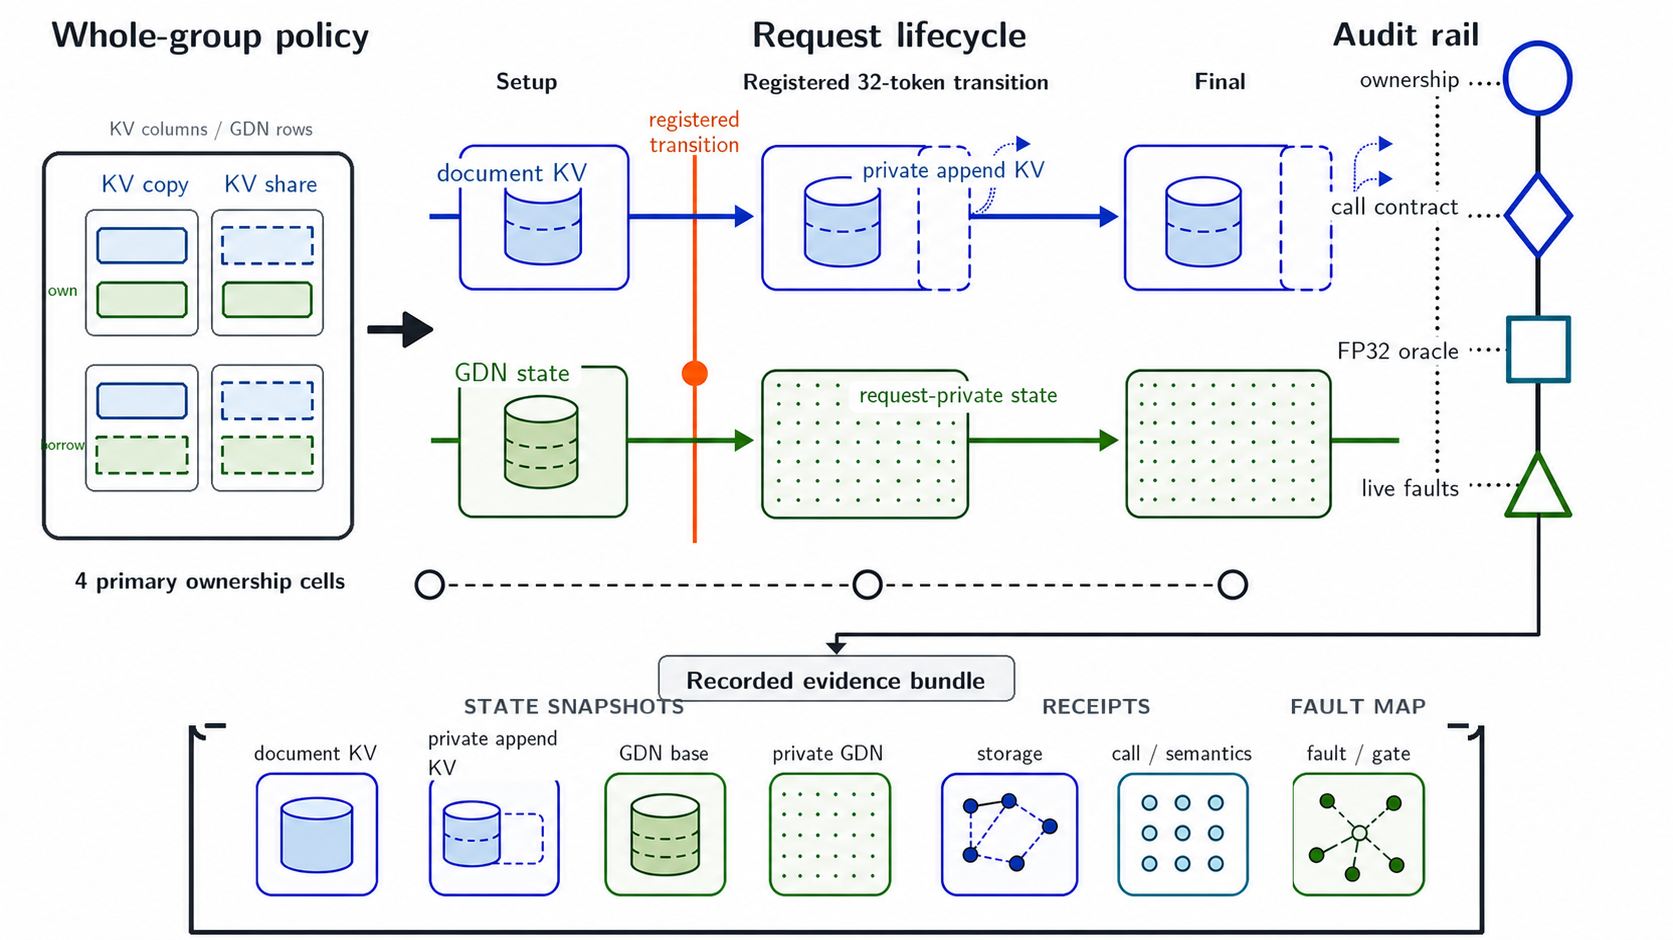
\includegraphics[width=0.98\textwidth]{figures/rr2_architecture_registered_transition.png}
  \caption{\method{} ownership factorial.  Four KV-by-GDN setup cells share
  immutable document state, keep append tails private, and rebind borrowed
  recurrent state at the registered transition.  The audit rail records
  lifecycle, storage, call/semantic, and fault-to-gate receipts.  This schematic
  details the validation component; it is not experimental evidence.}
  \label{fig:architecture}
\end{figure}

\begin{table}[H]
  \caption{Frozen primary-factorial execution geometry.  The eight ranks
  provide distinct books and query banks, not repeated stochastic
  measurements.}
  \label{tab:protocol}
  \centering
  \small
  \begin{tabular}{@{}p{0.25\linewidth}p{0.65\linewidth}@{}}
    \toprule
    Component & Frozen value \\
    \midrule
    Model & Qwen3.5-35B-A3B; 10 attention + 30 GDN layers \\
    Hardware & 8 $\times$ H20-3e; one book/rank \\
    Software & Python 3.11.13; PyTorch 2.11.0+cu129; Transformers 5.14.1; vLLM 0.26.0+cu129; Triton 3.6.0; CUDA 12.9 \\
    KV backend & vLLM fused attention; BF16/Q16; page 128 \\
    Document / query & 4,095 / 32 tokens; PG-19 train only \\
    Generation & 8 output tokens; 39 state-appended input tokens (32 query + 7 generated-token feedback) \\
    Resident counts & $1,8,32$; four KV-by-GDN ownership cells \\
    Primary schedule & all requests resident; batch-one sequential round-major calls on one CUDA stream/rank \\
    Validation & 96 factor configurations; separate memory/witness cells \\
    Fault campaigns & $N=2$; the primary all-gates-on campaign has nine live mutants with rebuilt controls; the target-gate-suppression campaign has nine fresh clean plus nine suppressed-gate cases on 8 H20s; the designer--executor-separated campaign has five new clean/mutant pairs on 5 H20s \\
    Historical regression & one previously encountered one-token alias defect; 8 ranks $\times$ 3 fresh $N=2$ lanes; 3 archived-coordinate reproductions + 5 additional frozen inputs; no mutation \\
    \bottomrule
  \end{tabular}
\end{table}

\begin{table}[H]
  \caption{Meaning of the V29 selected-cell evidence units.  Counts are per
  rank unless marked total; all belong to the same formal run.}
  \label{tab:v29-evidence-units}
  \centering
  \scriptsize
  \begin{tabular}{@{}p{0.21\linewidth}p{0.17\linewidth}p{0.54\linewidth}@{}}
    \toprule
    Unit & Count & Check and authorization \\
    \midrule
    Persistent sources & 60 & independently enumerated before the actual builder; exact object, storage, descriptor, and content remain fixed \\
    Selected anchors & 6/phase & preregistered persistent/request semantic rows; request-owned subset consumes the group-bound lineage capability \\
    Full live/serializer rows & 540/phase & $(1\text{ persistent}+8\text{ requests})\times60$ rows; live objects are re-enumerated and every serialized field, role, interval, content digest, and phase relation is checked \\
    Builder clone edges & 480 & $8\times60$ materialized destinations exhaust the captured persistent-rooted ledger and are direct \texttt{aten.clone} outputs \\
    Phase artifacts & 3 & setup, post-transition, and post-generation products are hash-bound, published to stable rank paths, and terminally reread \\
    Clean-memory context separation & 12 (96 total) & separate allocator-cell calls are all observed; zero selected-context overlaps mean the selected context did not enter them, not that the wrapper was absent or perturbation-free \\
    \bottomrule
  \end{tabular}
\end{table}

With field order (owner, request, layer, family, state), the six anchors are
$(\mathrm{Pers},\varnothing,0,\mathrm{rec},0)$,
$(\mathrm{Req},0,0,\mathrm{conv},0)$,
$(\mathrm{Req},0,1,\mathrm{conv},0)$,
$(\mathrm{Req},0,2,\mathrm{conv},0)$,
$(\mathrm{Req},0,2,\mathrm{rec},0)$, and
$(\mathrm{Req},1,0,\mathrm{rec},0)$.  The capability covers the five request
rows; the persistent row is their source anchor.

\begingroup
\footnotesize
\setlength{\LTpre}{0pt}
\setlength{\LTpost}{0pt}
\begin{longtable}{@{}>{\raggedright\arraybackslash}p{0.19\linewidth}>{\raggedright\arraybackslash}p{0.32\linewidth}>{\raggedright\arraybackslash}p{0.39\linewidth}@{}}
  \caption{Cohort-to-claim authorization.  Cohorts are never pooled; each row
  supports only the listed inference.}
  \label{tab:cohorts}\\
  \toprule
  Cohort & Frozen scope & Authorized claim / explicit exclusion \\
  \midrule
  \endfirsthead
  \multicolumn{3}{c}{\textit{Table~\ref{tab:cohorts} continued.}}\\
  \toprule
  Cohort & Frozen scope & Authorized claim / explicit exclusion \\
  \midrule
  \endhead
  \midrule
  \multicolumn{3}{r}{\textit{Continued on next page}}\\
  \endfoot
  \bottomrule
  \endlastfoot
  Primary ownership factorial & 8 books; $N=1,8,32$; four KV$\times$GDN cells; 8 decode steps & ownership lifecycle, cross-cell equivalence, selected attention oracle, live-mutant sensitivity, and four-cell allocator endpoints; not transfer or scheduler evidence \\
  Primary target-5 rerun & same frozen 8-rank, 96-configuration Qwen/H20 factorial; 209,920 attention and 635,520 GDN calls & per-call selected Triton kernel-cache artifact/configuration and eager-route binding at the declared fixed-stack scope; not device-side completion, driver/device, compiled-GDN, ATen/CUDA, performance, or cross-stack evidence \\
  Selected-cell live binding & same frozen 8-rank factorial; stronger hook active only for the $N=8$ shared-document/materialized-GDN cell; actual builder, production serializer, and direct clone lineage & 144 selected rows, 12,960 live-storage rows, 3,840 clone edges, and 24 phase artifacts pass; all 96 clean-memory calls have zero selected-context overlaps; not evidence for other cells or coordinates, malicious runtimes, framework independence, device binaries, or performance \\
  Fresh-process control & one independent $N=2$ process; one clean path and M1 & input reconstruction, cleanup, and one intended-gate reproduction; not pooled with the factorial \\
  Lifecycle transfer & 8 books; aligned 4,096-token prefix; $N=4$; two cancelled slots & exact outputs/state, zero-scrub, exact reuse, and stale-lease rejection on the same adapter; not scheduler, concurrency, or performance evidence \\
  Scheduler interleave & 8 books; $N=4$; page/prefix/tail geometries 64/3,985/17 and 128/4,033/65; cancel slot 3 after round 2 & deterministic request-step interleaving, zero-scrub, epoch change, exact reuse, uninterrupted-control equality, and three frozen scheduler-fault gates; not concurrent kernels, continuous-batching performance, detection rate, or production end-to-end correctness \\
  Independent preproducer slot census & frozen Qwen/H20 geometry and schedule; 180 slots/capture; two $N=2$ GDN-policy cells and three phases/cell & all 6 captures, 1,080 receiver rows, and 96,660 relations close; omission, duplication, and semantic-relabel controls fail closed; producer manifests/rows are not expected-set authority, but slot-ID-to-live-tensor binding, IPC, and paused capture remain trusted \\
  Dual-producer repeat & same frozen input/protocol and producer implementation; two fresh serial executions and four distinct out-of-process observers & both executions reproduce 1,080 semantic coordinates, byte digests, stable descriptors, and 96,660 relation labels at zero tolerance; not malicious-producer resistance, independent receiver model execution, or cross-stack evidence \\
  Falcon-H1 bounded transfer & \path{tiiuae/Falcon-H1-0.5B-Base}; Transformers 5.14.1/H20 naive path; $N=1,2$; separately executed official Transformers reference; persistent-Q16 and deep-materialized arms & 8/8 ranks, 96 generated-token and 96 full-vocabulary FP32-logit comparisons, 13,824 state rows across KV key/value, convolution, and Mamba2 recurrent families, 192 ownership checks, cross-arm/cross-$N$ relations, and registered controls pass; no performance, memory, quality, or other-stack evidence \\
  Bounded two-stream lifecycle & one H20; one 4,033-token document; two 16-token query requests at $N=2$; two host threads and distinct CUDA streams; pre-cancel and post-reclaim phases; cancellation after synchronization & positive call-interval overlap plus exact four lifecycle outputs, 20 logical-KV layer pairs, two GDN slot aggregates, ownership, scrub, and reuse; not simultaneous kernels, native continuous batching, in-flight cancellation, production scheduling, or performance \\
  GDN transition oracle & 1 frozen book/window; global model-layer indices 0, 10, 20, 38; 4 query tokens & clean recurrence outputs/states and four seeded wrong-transition rejections conditional on post-normalization inputs; not all GDN layers or end-to-end semantics \\
  Expanded captured-boundary numerical sweep & 2 distinct PG-19 inputs; all 10 attention layers and 12 of 30 GDN layers; 20 attention and 24 GDN clean rows plus one seeded control/row & captured-boundary numerical agreement and rejection of all 44 seeded wrong operators; not upstream-activation, independent-capture, full-model, or end-to-end validation \\
  Target-gate suppression matrix & 9 fresh clean + 9 target-suppressed cases; same fixed model/data/$N=2$; 8 distinct H20s & per-fault comparison with redundant audit gates, exact allowlisted production assertions, and token/FP32-logit equality; M8's injected sentinel is not a detector; not a blind-fault study or rate \\
  Designer--executor-separated faults & separate designer reads only the prior PDF; 5 new frozen $N=2$ clean/mutant pairs; 5 H20s; all gates enabled & all 5 clean gates pass and all 5 mutants fail first at their frozen primary predicate; per-fault sensitivity only, not a detection rate, natural-defect study, or cross-stack evidence \\
  Historical alias regression & one pre-discovery integration defect; 3 archived coordinates + 5 additional frozen inputs; fresh pre-fix, repaired, and materialized $N=2$ one-token lanes; 8 H20s & pre-fix binding gate and base violation with output/terminal-state equality, plus storage-clean exact repair; one retrospective defect only, not prevalence, recall, statistical replication, or cross-stack evidence \\
  Mac common-mode control & Apple M4 Pro; six documents/queries; five fresh MLX processes; vanilla dense plus CoMem BF16/Q8/Q4 at depth 7 & separates split-family agreement from agreement with vanilla dense; motivation only and separate from the H20 case \\
  H20 archival Store--F1 validation & 60 validation items from Qasper/2WikiMQA (30 each); dense, full-prefix, split Q16, frozen Q4/Q4/Q8, and two mixed policies & raw-first replay of Store, predictions, mean F1, paired bootstrap intervals, and fixed-case failure counts; not source-frozen regeneration, TTFT/TPOT/throughput, Recall, total memory, edge, or broad-benchmark evidence \\
  H20 deployment timing & source indices 6--9 from each of Qasper/2WikiMQA (8 items total), a subset of the 60-item validation cohort; no-cache dense recompute, full-prefix KV reuse, and CoMem Q8/Q4/mixed variants (six configurations total) with 3 timing repeats & same-stack retained-Store, TTFT, TPOT, tokens/s, and mean F1 comparison from a separate execution; not an independent replication, not pooled with the 60-item panel or primary factorial, and not scheduler/continuous-batching evidence \\
  Matched serving controls & 8 validation items from Qasper/2WikiMQA; vLLM 0.26 and SGLang 0.5.17 cache off/on plus 24 fixed-configuration HYPIC timing/quality cells; one H20-3e per item & within-block cache-hit, quality, and client-wall timing context; not pooled with in-process CoMem timings, not a cross-framework leaderboard, and not continuous-batching evidence \\
  HYPIC retained-state receipts & 8 Prefix Cache + 8 HYPIC cells on the same fixed TP=1 model/slice; receipt-instrumented SGLang lifecycle & median target-entry-owned physical tensor payload only; not timing, NVML/process memory, capacity, continuous batching, or ForkAudit ownership evidence \\
  Related-work operator transfer & Hydragen at $N=8/32$ on one captured layer-3 attention family; Palu on one layer with 8 calibration and 1 held-out PG19 row & same-checkpoint numerical and logical-state trade-offs only; not an all-layer implementation, LongBench/quality result, speedup claim, or jointly optimized system \\
  Local replay/storage accounting & one Apple Mac16,8 CPU host; three consecutive fixed-order runs without cache flush; manifest-only core package plus a serial profile with five locally complete supporting verifiers & local CPU replay wall time and logical file/byte counts only; not H20 capture, GPU perturbation, cold-start latency, online inference, compressed-upload size, or an uninstrumented-baseline delta \\
\end{longtable}
\endgroup

\begin{table}[H]
  \caption{Trace coverage and replay verdict for the seven contract targets in
  fresh frozen primary case.  Equality denotes canonical byte-digest identity
  as recorded.  Overall trace coverage is complete and all seven target
  verdicts pass at their declared fixed-stack scope.  A passing primary
  target verdict remains trace-relative and conditional on capture honesty,
  slot-ID-to-live-tensor binding, and the target boundary in Section~\ref{sec:contract}.
  The census removes producer rows as expected-set authority only for its bounded
  GDN cohort; supporting cohorts do not upgrade these targets to comprehensive
  system correctness.}
  \label{tab:witness}
  \centering
  \scriptsize
  \begin{tabular}{@{}>{\raggedright\arraybackslash}p{0.14\linewidth}p{0.11\linewidth}p{0.09\linewidth}>{\raggedright\arraybackslash}p{0.34\linewidth}>{\raggedright\arraybackslash}p{0.20\linewidth}@{}}
    \toprule
    Target & Trace coverage & Replay verdict & Decisive witness & Boundary \\
    \midrule
    Frozen identity & complete & pass & identical preflight/terminal source ledgers, terminal model rehash, and stable data/query/protocol/execution bindings & one primary-factorial formal run; the dual repeat recaptures only the bounded $N=2$ GDN cohort \\
    Prefix immutability & complete & pass & physical document-KV digests and GDN base guards across all three phases & one frozen configuration/geometry \\
    Private ownership & complete & pass & all-pairs request--base and request--peer range replay at the primary registered transition; actual-builder, serializer, and direct-clone receipts for the selected cell & pointer-free conservative intervals; stronger live binding covers only six selected rows per phase in one cell \\
    Tail-safe append & complete & pass & one-time 127-token private-tail copy before append & one partial-tail geometry \\
    Host-side launch/config. & complete & pass & per-call ID, selected kernel-cache artifact/configuration, autotuner outcome, GPU/stream, and post-return seal; source-bound GDN eager route & normal launcher return, not device completion; no driver/device, compiled-GDN, or ATen/CUDA attestation \\
    Cross-arm equivalence & complete & pass & tokens, shape/dtype-bound CPU-FP32 logit digests, logical KV, and GDN & one primary sequential schedule \\
    Cross-$N$ consistency & complete & pass & 288 all-arm adjacent-fan-out comparisons over 72 rank--query identities & relational, not an independent oracle \\
    \bottomrule
  \end{tabular}
\end{table}

Selected numerical oracles, constructed controls, lifecycle/scheduler checks,
the independent census and dual-producer repeat, bounded two-stream and Falcon
cohorts, and the historical reproduction are supporting checks rather than
additional contract targets.  Their captured-input, same-adapter,
process-separated-but-shared-IPC, second-configuration, and schedule boundaries
are reported separately.

\section{Pointer-Free Storage Witness Schema}
\label{app:storage-schema}

\paragraph{Target-to-record dependencies.}
The following matrix is normative.  I, L, E, and F denote the Identity,
Lifecycle, Execution, and Target/fault classes in Table~\ref{tab:normative-records};
parenthesized entries name mandatory fields.  Missing any marked field makes
that target open.  A preregistered geometry may make tail safety not applicable.
Target 5 additionally requires an exact per-call ID, selected kernel-cache
artifact/configuration, autotuner selection or explicit no-autotuner record,
assigned GPU/stream, and post-return seal; missing any applicable field leaves
target 5 open.  A missing F field invalidates the corresponding fault row,
but does not change the separately evaluated seven-target witness.

\begin{center}
\scriptsize
\setlength{\tabcolsep}{2.5pt}
\begin{tabular}{@{}p{0.13\linewidth}p{0.17\linewidth}p{0.17\linewidth}p{0.20\linewidth}p{0.08\linewidth}p{0.14\linewidth}@{}}
\toprule
Target & I & L & E & F & Blind predicate \\
\midrule
Frozen identity & code, model, data, protocol; role map & --- & --- & N/A & exact bytes and complete roles \\
Prefix immutability & document/base roles; start digests & setup and final guards & canonical content digests & N/A & start $=$ final \\
Private ownership & request/base/private roles & setup, registered-transition, final bindings & normalized storage ranges & N/A & non-vacuous all-pairs disjointness \\
Tail-safe append & page geometry; document/private roles & first append event & ordered append and copied-tail receipt & N/A & one private copy before write \\
Host-side launch/config. & callable, source, protocol, selected artifact/config. & post-return seal; GPU/stream assignment & ordered call, query, mask, position, append, scale, autotuner outcome, eager route & N/A & exact per-call binding; no fallback or route contamination \\
Cross-arm equivalence & factor, query, and schedule identities & final bindings & token, logit, logical-KV, GDN records & N/A & canonical semantic equality \\
Cross-$N$ consistency & query and fan-out identities & --- & the same canonical semantic records & N/A & smallest-$N$ equals each larger $N$ \\
Fault sensitivity (supporting) & frozen target/gate map & matched-control rebuild and cleanup & injected outcome and failed predicates & required & target, injection, expected gate, outcome \\
\bottomrule
\end{tabular}
\end{center}

Each tensor-view row has the exact fields
\texttt{storage\_id}, \texttt{shape}, \texttt{stride},
\texttt{storage\_offset}, \texttt{dtype}, \texttt{device},
\texttt{storage\_nbytes}, \texttt{tensor\_nbytes}, and
\texttt{content\_sha256}; absolute addresses are forbidden.  Within each
phase, the producer assigns \texttt{storage-0000}, \texttt{storage-0001},
and so on in first-observation order to backing storages.  Reusing an ID with
a different device or storage size is invalid.  Phase capture IDs are unique,
whereas request and persistent lifecycle-guard IDs must remain stable across
setup, the registered transition, and final generation.

Let element size be $e$, storage offset $o$, shape $s_i$, and stride $t_i$.
The independent replay initializes $m=M=o$ and, for every dimension, computes
\begin{equation}
  d_i=(s_i-1)t_i,\qquad
  m\mathrel{+}=\min(d_i,0),\qquad
  M\mathrel{+}=\max(d_i,0).
\end{equation}
The conservative half-open byte interval is
\begin{equation}
  I=[em,\,e(M+1)),
\end{equation}
which must be non-negative and contained in \texttt{storage\_nbytes}; also
\texttt{tensor\_nbytes}$=e\prod_i s_i$.  Two rows overlap iff their normalized
storage IDs match and $I_a^{\mathrm{start}}<I_b^{\mathrm{end}}$ and
$I_b^{\mathrm{start}}<I_a^{\mathrm{end}}$.  Exact aliasing additionally
requires equality of interval, geometry, dtype/device, storage and tensor
sizes, and content digest.  For correctly live-bound rows at one capture, if
represented views sharing physical backing receive the same normalized ID and
their shape, stride, offset, and element size exactly describe affine-strided
views, $I$ contains every touched byte.  The overlap test then cannot miss a
shared byte between represented rows, although interleaving may cause false
positives.  Omitted rows, between-capture changes, and wrapper or storage-ID
violations remain outside the claim.

At setup, every recurrent-state coordinate must either exactly alias the
persistent state (borrowed-base arm) or be disjoint from it (materialized
arm).  At the primary registered 32-token transition boundary, a completed
request's 60 mutable rows must be disjoint from the base and every peer;
incomplete borrowed requests must
remain exact aliases.  At final, all request-local GDN states must be disjoint
from the persistent GDN base and every peer; document KV remains intentionally
shared.
Independent binding-token receipts additionally require unchanged tokens for
incomplete requests and changed binding/storage tokens for completed requests.
The package applies this schema to all 96 timelines and 288 phase artifacts;
nine adversarial tests cover exact aliasing, partial overlap, adjacent
intervals, negative strides, conflicting ID reuse, pointer injection,
capture/guard reuse, and cross-coordinate request--base and request--peer
aliasing.

\section{Executed Fault Rows and Invariant Map}
\label{app:invariants}

The row-level campaign is kept out of the main paper because it supports
diagnosis and audit coverage rather than a separate headline result.
Separately, the CPU governance suite passes 17 tests and rejects 28 explicit
serialized-artifact tamper cases plus its registered helper/launcher faults.
That result concerns schema and orchestration fail-closure only; it is not GPU
semantic or performance evidence.
\begin{table}[H]
\caption{Separate primary all-gates-on reference. Every separately rebuilt matched-clean cell passed; every mutant reached its target gate fixed before execution and was restored before disposal.}
\label{tab:rr2-mutants}
\centering\footnotesize
\begin{tabular}{@{}clll@{}}
\toprule
ID & Injected live fault & Expected/observed gate & Primary outcome \\
\midrule
M1 & reservation alias & \texttt{KV\_RESERVATION\_DISJOINT} & target gate reached \\ 
M2 & sequence swap & \texttt{KV\_SEQUENCE\_ID} & target gate reached \\ 
M3 & omit tail COW & \texttt{KV\_TAIL\_COW} & target gate reached \\ 
M4 & GDN--base alias & \texttt{gdn\_completed\_vs\_base\_disjoint} & target gate reached \\ 
M5 & GDN peer alias & \texttt{gdn\_completed\_vs\_peers\_disjoint} & target gate reached \\ 
M6 & position off-by-one & \texttt{POSITION\_CANONICAL\_VALUES} & target gate reached \\ 
M7 & materialized mask & \texttt{MASK\_CONTRACT} & target gate reached \\ 
M8 & wrong callable & \texttt{KERNEL\_CALLABLE\_ID} & target gate reached \\ 
M9 & dense KV view & \texttt{KV\_PAGED\_VIEW} & target gate reached \\ 
\bottomrule
\end{tabular}
\end{table}


\begin{table}[H]
\caption{Same-system outcomes for nine designed faults.  The primary campaign
enables all gates; a separate target-gate-suppression campaign suppresses only
the named gate.
``Same'' is exact and ``N/O'' an earlier stop.  Rows are not a detection rate;
M8's injected sentinel is not a production detector.}
\label{tab:first-gate-localization}
\centering\scriptsize
\setlength{\tabcolsep}{2.6pt}
\begin{tabular}{@{}p{0.19\linewidth}p{0.12\linewidth}p{0.39\linewidth}p{0.18\linewidth}@{}}
\toprule
Fault / target contract & All gates on & With target gate suppressed & Token / FP32 logits \\
\midrule
M1 Reservation ownership & target gate & completes & Same / Same \\
M2 Sequence binding & target gate & completes & Same / Same \\
M3 Tail COW & target gate & other audit: active-block ownership & N/O / N/O \\
M4 GDN base isolation & target gate & other audit: peer isolation & N/O / N/O \\
M5 GDN peer isolation & target gate & completes; logits change ($L_\infty=0.75$, rel. $L_2=0.0314$) & Same / Changed \\
M6 Positions & target gate & completes & Same / Same \\
M7 Mask contract & target gate & completes & Same / Same \\
M8 Callable identity & target gate & injected payload sentinel & N/O / N/O \\
M9 Paged-KV view & target gate & paired-view production assertion & N/O / N/O \\
\bottomrule
\end{tabular}
\end{table}


\paragraph{Designer--executor-separated fault detail.}
The five fixed per-fault outcomes summarized in the main text are shown below;
they remain constructed controls rather than a defect-population sample.
\begin{table}[H]
\caption{Designer--executor-separated constructed fault outcomes.  A separate
designer saw only a frozen earlier manuscript PDF and fixed all five
definitions, loci, payloads, clean requirements, and expected first predicates
before executor preparation or candidate output.  The cases are separated from
executor preparation and outcome inspection, not from the predicate vocabulary.  All
matched clean cases pass; every mutant completes its
registered horizon and is rejected first by the frozen primary predicate.
Semantic comparisons are secondary: ``Same'' means canonical exact equality
with the matched clean case, KV/GDN denote terminal logical state, and ``N/C''
means full-logit call cardinality is not comparable.  These five fixed outcomes
are not a population detection rate.}
\label{tab:r33-fresh-heldout}
\centering\scriptsize
\setlength{\tabcolsep}{2.5pt}
\begin{tabular}{@{}p{0.18\linewidth}p{0.22\linewidth}p{0.27\linewidth}p{0.22\linewidth}@{}}
\toprule
Frozen fault & Isolated mutation & First failed predicate & Tokens / logits / KV / GDN \\
\midrule
HF01 delayed tail detach & append write precedes the otherwise present tail copy & tail-copy-before-first-write & Same / Same / Same / Same \\
HF02 inactive-lane scribble & one bit in the unused lane of a shared physical K page & physical-prefix immutability & Same / Same / Same / Same \\
HF03 duplicate commit & one correct feedback call commits twice; first output discarded & ordered-call cardinality & Same / N/C / Changed / Changed \\
HF04 effective-scale drift & first registered attention scale is exactly doubled & attention effective scale & Changed / Changed / Changed / Changed \\
HF05 stale GDN binding token & storage correctly rebinds; lifecycle token remains stale & completed binding-token advance & Same / Same / Same / Same \\
\bottomrule
\end{tabular}
\end{table}


\begin{table}[H]
\caption{Representative failure families and intended checks.  Rows naming
M1--M9 refer to the nine executed primary-factorial live mutants; the other
rows summarize schema, relational, numerical, or replay checks.  None is a
complete oracle.}
\centering\small
\begin{tabular}{@{}p{0.23\linewidth}p{0.66\linewidth}@{}}
\toprule
Check family & Intended sensitivity and observed boundary \\
\midrule
Frozen identity & wrong model/data/query bank, changed protocol, stale shard (schema adversaries)\\
Prefix immutability & M3 omits partial-tail COW; physical document digest and ownership gates fail\\
Private ownership & M1 reservation alias, M4 request--base GDN alias, M5 request--peer GDN alias\\
Sequence/view binding & M2 sequence swap and M9 dense-KV replacement\\
Host-side selected launch/configuration & M6 position offset, M7 materialized mask, M8 wrong callable\\
Factorial exactness & behavior changes when either KV or GDN setup ownership changes\\
Bounded numerical oracle & numerical error in a selected fused full-attention result\\
Raw replay & internally inconsistent trajectory, storage, allocator, or aggregate fields\\
\bottomrule
\end{tabular}
\end{table}

The primary all-gates-on execution is a first-gate localization study.  Every registered gate
fires before the injected path produces a post-injection token, logit,
logical-KV digest, or GDN digest; its output cells are therefore N/O rather
than misses.
Lifecycle/ownership/storage receipts supply the first gate for M1 and M3--M5;
request-binding/call receipts supply it for M2 and M6--M9.  The full audit
rejects all nine at their predeclared gates under passing matched controls.
The separate target-gate-suppression matrix then suppresses one named gate per mutant while leaving
the remaining observers active.  It provides the per-fault comparison in
Table~\ref{tab:first-gate-localization}, but does not estimate a population
rate, unseen-fault coverage, or false-positive rate.

\section{Relation to Prior Work and Audit Obligations}
\label{app:novelty-boundary}

\begin{table}[H]
  \caption{Primary-source positioning.  ``Evidence focus'' describes what the
  cited work evaluates; it is not a claim that the work lacks all other checks.}
  \label{tab:closest}
  \centering
  \footnotesize
  \begin{tabular}{@{}p{0.16\linewidth}p{0.28\linewidth}p{0.43\linewidth}@{}}
    \toprule
    Work & Primary mechanism & Evidence focus / relation to this work \\
    \midrule
    PagedAttention & Paged KV allocation and sharing~\citep{kwon2023pagedattention} & Serving throughput and memory utilization; supplies the block-sharing substrate. \\
    SGLang / Prompt Cache & Prefix reuse in structured or modular prompts~\citep{zheng2024sglang,gim2024promptcache} & Runtime performance and output behavior; establish reuse and positional handling as prior art. \\
    CoMem & One persistent residual per token at split $j$; bounded selection; suffix replay~\citep{liu2026comem,liu2026understanding} & Supplies the split-replay foundation; we do not claim that primitive as new. \\
    \qcomem{} (ours) & Joint low-bit split residual and required lower KV/convolution/recurrent state & Adds complete hybrid-state packing, a capacity--latency--quality evaluation, and an auditable request-local ownership boundary; not a model-weight compressor or production scheduler. \\
    Marconi & Admission and eviction for hybrid-model prefixes~\citep{pan2025marconi} & Hybrid cache hit rate and time to first token; closest state-heterogeneous caching system, but a different policy-level contribution. \\
    SCBench & Lifecycle-oriented KV-cache benchmark~\citep{li2025scbench} & Breadth over tasks and cache phases; exposes breadth absent from our bounded declared configurations. \\
    MT-DLComp / CRADLE & Metamorphic compiler testing and cross-backend differential checking~\citep{xiao2022metamorphic,pham2019cradle} & Direct testing precedents; our audit adds ownership witnesses and a layerwise dense oracle, but not an independent end-to-end backend. \\
    DNNMem & Component-wise GPU-memory accounting~\citep{gao2020dnnmem} & Supports denominator separation; it is an estimator, not a request-ownership audit. \\
    \method{} & Typed, phase-indexed ownership/call/accounting trace with explicit coverage semantics & Validates the ownership component through a mutation-tested KV-by-GDN factorial, bounded host-side call receipts, a preproducer expected-slot census, numerical sweeps, and one bounded Falcon-H1 comparison; it is not a security attestation or general end-to-end correctness oracle. \\
    \bottomrule
  \end{tabular}
\end{table}

\begin{table}[H]
\caption{Closest established precedent for each audit obligation.  The final
column states the narrower integration contributed by \method{}; it does not
claim that any individual mechanism is new.}
\centering\scriptsize
\begin{tabular}{@{}p{0.18\linewidth}p{0.31\linewidth}p{0.42\linewidth}@{}}
\toprule
Audit obligation & Closest established precedent & Integrated obligation in this work \\
\midrule
Frozen identity & Controlled variants in metamorphic and differential testing~\citep{chen2018metamorphic,xiao2022metamorphic,pham2019cradle} & Bind model, data, query bank, callable contract, and protocol bytes to every ownership receipt. \\
Document immutability and tail COW & PagedAttention block sharing and copy-on-write for shared prefixes~\citep{kwon2023pagedattention} & Replay physical document pages, padding, active tables, and the partial-tail detach event. \\
Recurrent-state ownership & Hybrid recurrent states and their in-place update constraint~\citep{yang2025gateddeltanet,pan2025marconi} & Witness request--base and request--peer ranges before and after the frozen schedule's registered transition boundary. \\
Host-side selected launch/configuration & Cross-backend differential checking exposes implementation-dependent behavior~\citep{pham2019cradle} & Hold the backend fixed; record callable, positions, mask, scale, and append history; and bind the selected Triton kernel-cache artifact/configuration per attention call while keeping GDN at an explicit eager-route boundary. \\
Cross-arm and cross-$N$ relations & Metamorphic relations over semantics-preserving transformations~\citep{chen2018metamorphic,xiao2022metamorphic} & Treat ownership policy and resident fan-out as transformations that must preserve registered request observables. \\
Bounded numerical oracle & Independent backend comparison~\citep{pham2019cradle} & Reconstruct selected attention inputs for dense IEEE-FP32 math and selected post-normalization GDN inputs for a candidate-import-free NumPy recurrence. \\
Memory denominators & Component-wise GPU-memory accounting~\citep{gao2020dnnmem} & Keep page geometry, allocator current/peak, and unmeasured process/service capacity as separate claim domains. \\
\bottomrule
\end{tabular}
\end{table}

\FloatBarrier

\section{Supporting Control Experiments}
\label{app:controls}

\paragraph{Mac common-mode motivation.}
The archival Apple-M4-Pro control is kept unpooled from the H20 experiments and
serves only to show why split-family agreement does not replace a dense or
independently implemented oracle.
\begin{table}[H]
\caption{Unpooled Mac motivation context (Apple M4 Pro, five fresh MLX processes; median over 30 query executions at split depth 7). Vanilla dense is the external reference. \qcomem{} BF16/Q8/Q4 variants use the same selected documents. Store size is the six-document residual corpus; online time includes query Write, dequantization, and suffix Read. This small teacher-forced demonstration set is not primary ForkAudit evidence and supports no cross-hardware or production-speed claim.}
\label{tab:mac-motivation}
\centering\scriptsize
\setlength{\tabcolsep}{2.7pt}
\begin{tabular}{@{}lrrrr@{}}
\toprule
Method & Store (MiB) & Online (ms) & Speedup & Top-1 vs. dense \\
\midrule
Vanilla dense prompt & -- & 194.70 & 1.00$\times$ & 100.00\% \\
\qcomem{} BF16 split & 1.998 & 168.88 & 1.15$\times$ & 71.89\% \\
\qcomem{} Q8 split & 1.061 & 169.17 & 1.15$\times$ & 71.89\% \\
\qcomem{} Q4 split & 0.562 & 169.25 & 1.15$\times$ & 71.89\% \\
\bottomrule
\end{tabular}
\vspace{0.5mm}
\parbox{0.98\linewidth}{\scriptsize Q8/Q4 retain 100\% top-1 agreement with the BF16 split path, yet all split rows inherit only 71.89\% agreement with vanilla dense. The speed column is a small teacher-forced mechanism benchmark, not production RAG throughput.}
\end{table}


\paragraph{Historical alias regression and repair.}
The pre-fix, repaired, and materialized lanes isolate one previously observed
recurrent-state alias.  This is a fixed mechanism study, not a natural-bug
frequency or detector-recall estimate.
\begin{table}[H]
\caption{Retrospective reproduction and repair of one historical alias
regression.  Ranks 0--2 reuse three archived input coordinates; ranks 3--7
are additional frozen inputs, not additional defects or statistical
replicates.  Semantic columns compare each path with a fresh materialized
control.  ``Base inv.'' is within-path persistent-base immutability, retained
as a conventional state-invariant catch.}
\label{tab:r35-historical-alias}
\centering\scriptsize
\setlength{\tabcolsep}{2.1pt}
\begin{tabular}{@{}>{\raggedright\arraybackslash}p{0.14\linewidth}>{\raggedright\arraybackslash}p{0.08\linewidth}>{\raggedright\arraybackslash}p{0.20\linewidth}p{0.075\linewidth}p{0.085\linewidth}p{0.09\linewidth}p{0.075\linewidth}p{0.07\linewidth}@{}}
\toprule
Coordinates & Path & Ownership result & Token & FP32 logits & Request GDN & Logical KV & Base inv. \\
\midrule
Archived (3) & Pre-fix & binding gate 3/3 & exact 3/3 & exact 3/3 & exact 3/3 & exact 3/3 & fail 3/3 \\
Archived (3) & Repaired & storage-clean 3/3 & exact 3/3 & exact 3/3 & exact 3/3 & exact 3/3 & pass 3/3 \\
Additional (5) & Pre-fix & binding gate 5/5 & exact 5/5 & exact 5/5 & exact 5/5 & exact 5/5 & fail 5/5 \\
Additional (5) & Repaired & storage-clean 5/5 & exact 5/5 & exact 5/5 & exact 5/5 & exact 5/5 & pass 5/5 \\
\bottomrule
\end{tabular}
\end{table}


\paragraph{Primary allocator endpoints.}
The four ownership cells use one frozen post-priming allocator denominator and
are kept separate from deployment Store.
\begin{table}[H]
\caption{Primary 8$\times$H20-3e allocator results at $N=32$ (median across ranks; rank values coincide). Full-copy is the factorial control; the paged-prefix row is the closest same-stack prefix-sharing baseline. The remaining rows isolate recurrent-base ownership. All cells retain the persistent document source. Values are GiB above the frozen post-priming baseline; generation increment is the additional peak above allocation present at generation start.}
\label{tab:rr2-memory}
\centering\scriptsize
\setlength{\tabcolsep}{2.6pt}
\begin{tabular}{@{}p{0.25\linewidth}p{0.25\linewidth}rrr@{}}
\toprule
Empirical arm & KV / GDN setup & Final & Peak & Gen. incr. \\
\midrule
Full-copy factorial control & Full-copy KV / Materialized GDN base & 4.901 & 4.920 & 0.019 \\
GDN ownership ablation & Full-copy KV / Borrowed GDN base & 4.890 & 4.907 & 1.951 \\
Paged-prefix baseline & Shared-doc KV / Materialized GDN base & 2.229 & 2.843 & 0.019 \\
Audited hybrid fork & Shared-doc KV / Borrowed GDN base & 2.229 & 2.843 & 1.950 \\
\bottomrule
\end{tabular}
\end{table}


\paragraph{Published systems context.}
Table~\ref{tab:published-context} reports each cited system only in its native
protocol and keeps all non-commensurate metrics outside our matched panels.
This unpooled table is literature context, not ForkAudit evidence.
\begin{table}[H]
\caption{Unpooled published-systems context in each paper's native protocol.  These values show the scale and evaluation breadth of related systems, \emph{not} a cross-paper leaderboard or ForkAudit evidence: models, hardware, batching, baselines, and metrics differ.  Consequently, no row is merged with our same-stack H20 Table~\ref{tab:h20-deployment}, and the absence of a common score must not be read as a negative result.}
\label{tab:published-context}
\centering\scriptsize
\setlength{\tabcolsep}{2.5pt}
\begin{tabular}{@{}>{\raggedright\arraybackslash}p{0.15\textwidth}>{\raggedright\arraybackslash}p{0.28\textwidth}>{\raggedright\arraybackslash}p{0.265\textwidth}>{\raggedright\arraybackslash}p{0.245\textwidth}@{}}
\toprule
System & Native method and study setting & Reported efficiency in its native protocol & Quality and comparability boundary \\
\midrule
PagedAttention / vLLM~\citep{kwon2023pagedattention} & Paged KV allocation plus serving engine\newline \textit{Setting:} LLaMA-7B on A10G and LLaMA-13B on A100-40GB; vLLM serving engine & 2--4$\times$ serving throughput at similar latency vs. FasterTransformer/Orca & No common LongBench F1; exact cache-management method \\
Prompt Cache~\citep{gim2024promptcache} & Modular attention-state reuse\newline \textit{Setting:} Llama2/MPT/Falcon; RTX 4090, A40, and A100; HuggingFace-style prototype & 1.5--3.1$\times$ TTFT (CPU-resident modules); 3.7--11.7$\times$ (GPU-resident) on its 12-dataset LongBench suite & LongBench accuracy evaluated, but with different models and hardware \\
SGLang / RadixAttention~\citep{zheng2024sglang} & Prefix reuse plus structured-program runtime\newline \textit{Setting:} Llama-7B/Mixtral-8x7B and structured programs; A10G/A100; SGLang & Up to 6.4$\times$ throughput vs. prior inference systems & Application-suite result; no common LongBench F1 \\
ChunkAttention~\citep{ye2024chunkattention} & Prefix-aware KV chunks and attention kernel\newline \textit{Setting:} attention microbenchmarks; mainly A100-80GB, plus A100-40GB/RTX 4090; CUDA 11.8 & 3.2--4.8$\times$ attention-kernel speedup for 1K--4K shared prompts & Kernel result; no end-to-end common task score \\
Hydragen~\citep{juravsky2024hydragen} & Exact batched shared-prefix attention\newline \textit{Setting:} CodeLlama-13B/34B shared-prefix batches; A100 (with H100/L40S microbenchmarks); custom HuggingFace runtime & Up to 32$\times$ CodeLlama-13B end-to-end throughput in large shared-prefix batches & Exact attention construction; different model and batching regime \\
Palu~\citep{chang2025palu} & Low-rank latent KV with reconstruction/fusion\newline \textit{Setting:} Llama/Mistral/LongChat quality studies; Llama-2-7B latency on one RTX 4090; HuggingFace plus custom kernels & 50\% KV compression and up to 1.89$\times$ RoPE-attention speedup; up to 2.91$\times$ with quantization & Llama/Mistral/LongChat native study; our bounded Qwen3.5 operator transfer is reported separately \\
Preble~\citep{srivatsa2025preble} & Distributed prompt-sharing scheduling\newline \textit{Setting:} Mistral-7B/Llama-3-70B request traces; two--eight GPUs across A6000/H100 clusters; distributed serving & 1.5--14.5$\times$ average-latency and 2--10$\times$ p99-latency improvement & Distributed serving traces; no common task score \\
Marconi~\citep{pan2025marconi} & Admission/eviction for hybrid-model prefixes\newline \textit{Setting:} Attention--Mamba2 7B geometry; LMSys/ShareGPT/SWE-bench traces; CloudLab policy simulation & Up to 34.4$\times$ token-hit rate and up to 71.1\% or 617 ms lower TTFT & Hybrid models and trace-driven policy study; no common LongBench F1 \\
KVTuner~\citep{li2025kvtuner} & Offline sensitivity-aware search over layer-wise mixed-precision KV bit pairs\newline \textit{Setting:} Llama-3.1-8B-Instruct and Qwen2.5-7B-Instruct; mathematical- and general-reasoning suites & Nearly lossless 3.25-bit mixed-precision KV for Llama-3.1-8B-Instruct and 4.0-bit for Qwen2.5-7B-Instruct; up to 21.25\% higher maximum inference throughput vs. KIVI-KV8 & Layer-wise bit search for a dense KV cache; it does not quantize a split residual or recurrent state, and no common Qwen3.5 slice exists \\
HYPIC~\citep{liu2026hypic} & Position-independent caching for hybrid full/linear-attention models\newline \textit{Setting:} Qwen3.5-35B-A3B main panels at TP=2 on 8 H20-3e; SGLang 0.5.14 & 3.25$\times$ lower TTFT on average and 1.66$\times$ higher QPS over Prefix Cache & Four models/five workloads; our same-slice TP=1 timing and retained-state controls are reported separately \\
\bottomrule
\end{tabular}
\end{table}


\paragraph{Same-checkpoint transfer detail.}
Table~\ref{tab:related-transfer} is the matched complement to the published
context table: it uses our frozen Qwen3.5 checkpoint and H20-3e, binds the
official Hydragen and Palu source revisions, and independently replays all raw
operator sidecars.  Because it does not execute all layers or LongBench, it is
kept separate from Table~\ref{tab:h20-deployment}.
\begin{table}[H]
\caption{Bounded same-checkpoint H20 transfers.  Hydragen uses frozen Qwen3.5
layer-3 post-RoPE attention; Palu uses eight 256-token PG19 calibration rows
and one disjoint held-out row.  Errors are relative $\ell_2$ against the
matched uncompressed operator; state ratios are logical selected-operator
ratios, not process memory or end-to-end results.}
\label{tab:related-transfer}
\centering\scriptsize
\setlength{\tabcolsep}{2.8pt}
\begin{tabular}{@{}p{0.16\linewidth}p{0.12\linewidth}p{0.25\linewidth}p{0.20\linewidth}p{0.18\linewidth}@{}}
\toprule
Port & Setting & Matched numerical result & Logical state result & Timing / boundary \\
\midrule
Hydragen port & $N=8$ & Hydragen--dense rel. $\ell_2=0.00255$ & 8.50 vs. 64.48 MiB ($7.59\times$ smaller) & 0.287 vs. 0.0965 ms; no speedup \\
Hydragen port & $N=32$ & Hydragen--dense rel. $\ell_2=0.00262$ & 10.00 vs. 257.94 MiB ($25.80\times$ smaller) & 0.290 vs. 0.259 ms; no speedup \\
\midrule
Palu port & rank 64/head & held-out K/V $0.487/0.549$ (plain $0.711/0.839$) & 512 vs. 2,048 B/token ($4.00\times$ smaller) & projection only; no fused kernel \\
Palu port & rank 128/head & held-out K/V $0.317/0.364$ (plain $0.543/0.668$) & 1,024 vs. 2,048 B/token ($2.00\times$ smaller) & projection only; no fused kernel \\
Palu port & rank 192/head & held-out K/V $0.149/0.194$ (plain $0.341/0.459$) & 1,536 vs. 2,048 B/token ($1.33\times$ smaller) & projection only; no fused kernel \\
\bottomrule
\end{tabular}
\vspace{0.5mm}
\parbox{0.97\textwidth}{\footnotesize Hydragen avoids prefix replication but
has no speedup here.  Palu improves over plain SVD, but residual error forbids
an end-to-end quality claim.  Neither is a jointly optimized combined system.}
\end{table}


\subsection{Extended Deployment and Serving Context}
\label{app:illustrative-store}

Table~\ref{tab:qcomem-tradeoff} isolates the matched Transformers block used for
the main \qcomem{} claim.  The expanded table below repeats that block only to
place separately measured SGLang/HYPIC context beside it.  The blocks use
different runtimes and harnesses, so timing and F1 are interpreted within block
and are not pooled.  These serving controls are not \method{} validation
evidence and do not establish robust quality preservation.

\begin{table}[!ht]
\caption{Illustrative same-checkpoint H20 retained Store and mean-F1 point
estimates on an eight-item Qasper/2WikiMQA slice.  All rows use
Qwen3.5-35B-A3B, one H20-3e per item, a 4,096-token cap, greedy decoding, and
at most 32 generated tokens.  The Transformers (three repeats/item) and
HYPIC~\citep{liu2026hypic} blocks are unpooled; HYPIC timing/F1 and Store use
separate 24- and 16-cell TP=1 cohorts.  Timing is compared only within blocks;
no robust-quality, capacity, or ForkAudit-ownership claim is made.}
\label{tab:h20-deployment}
\centering\scriptsize
\setlength{\tabcolsep}{3.2pt}
\begin{tabular}{@{}llrrrrr@{}}
\toprule
Method & Persistent state & Store (MiB) & TTFT (s) & TPOT (ms) & tok/s & F1 \\
\midrule
\multicolumn{7}{@{}l}{\emph{Transformers 5.14.1 in-process deployment cohort}}\\
No-cache dense recompute & -- & -- & 0.649 & 648.75 & 1.36 & 39.42 \\
Full-prefix KV cache & Q16 & 140.34 & 0.163 & 54.11 & 13.38 & 39.14 \\
\qcomem{} state & Q8 & \textbf{15.89} & 0.673 & 55.44 & 7.15 & 39.14 \\
\qcomem{} mixed state & Q4/Q4/Q8 & 10.01 & 0.674 & 54.97 & 7.19 & 39.01 \\
\qcomem{} per-layer mixed & mixed & \textbf{9.74} & 0.673 & 55.07 & 7.19 & 39.11 \\
\qcomem{} state & Q4 & 8.41 & 0.674 & 55.02 & 7.19 & 36.09 \\
\midrule
\multicolumn{7}{@{}l}{\emph{HYPIC commit 98147c0 timing/F1; receipt-instrumented Store; SGLang 0.5.14, TP=1}}\\
Official HYPIC code: full recompute & -- & -- & 0.217 & 49.21 & 14.77 & 39.14 \\
Official HYPIC code: prefix cache & Radix prefix & 139.53 & 0.072 & 50.15 & 19.07 & 39.14 \\
HYPIC (transition + seam 8) & segment transition & 324.09 & 0.101 & 52.13 & 17.67 & 39.63 \\
\bottomrule
\end{tabular}
\vspace{0.5mm}
\parbox{0.97\textwidth}{\scriptsize Bold marks the two illustrative Store--F1 points; these are not a headline validation result.  Relative to full-prefix Q16, Q8/per-layer mixed reduce Store $88.68\%$/$93.06\%$; unrounded mean-F1 deltas are $0.000$/$-0.022$ ($39.115$ vs. $39.137$ for mixed).  ``--'' means no retained entry; Q16 is the unpacked reference, BF16 for the residual and attention KV and the stack's native FP32 for GDN recurrent state.  Full-prefix Q16 is \qcomem{}'s matched semantic comparator; the archived rows show no-cache recompute sharing the same document/query boundary but emitting different greedy token sequences on a few items.  Q4/Q4/Q8 gives residual/attention/linear bits.  The per-layer policy (Q4 residual, layer bits $[8,8,4,4,8,8,8]$) was selected on a separate, disjoint four-item calibration set and frozen before this eight-item validation.  Store is median retained-document tensor payload and excludes metadata, pools, process deltas, and capacity.  Published HYPIC panels use TP=2; this adaptation uses TP=1.}
\end{table}


\paragraph{Matched serving-framework and HYPIC context.}
Table~\ref{tab:serving-controls} gives separately timed vLLM and SGLang
cache-off/on controls plus the official-code HYPIC Full Recompute, Prefix
Cache, and full HYPIC arms under the shared Qwen3.5 streaming boundary.  It
remains a timing/quality-only panel and authorizes only within-framework
interpretation; the separate 16-cell retained-state receipt cohort appears in
Table~\ref{tab:h20-deployment}.
vLLM and SGLang each record 8/8 prefix hits and preserve 8/8 cache-off
predictions.  Within its TP=1 block, HYPIC gives 39.63, 0.101 s, and 17.67
tokens/s; published Qwen3.5 panels use TP=2, so this is an adaptation.  Its 24
timing cells bind a 4,404-entry terminal artifact ledger.  Across the
16 retained-state cells, Prefix Cache retains a median 139.53 MiB and HYPIC
retains 324.09 MiB; Prefix Cache and HYPIC retain $8.78\times$ and
$20.39\times$ as much Store as CoMem Q8, respectively, under the separate
Store estimand.  This remains single-stream; it does not measure continuous
batching.
\begin{table}[H]
\caption{Unpooled timing/quality-only serving context on Qwen3.5 and the same eight-item Qasper/2WikiMQA slice.  Each row uses one H20-3e per item, a 4,096-token cap, greedy decoding, and at most 32 generated tokens.  Times are OpenAI-compatible streaming client wall-clock; F1 is the eight-item mean.  Hit is interpreted only against the disabled/full-recompute reference inside each framework block.  No cross-framework speedup, retained-state, scheduler-throughput, capacity, or broad-quality claim is made.}
\label{tab:serving-controls}
\centering\scriptsize
\setlength{\tabcolsep}{4.0pt}
\begin{tabular}{@{}llrrrrc@{}}
\toprule
Framework & Prefix reuse & F1 & TTFT (s) & TPOT (ms) & tok/s & Hit \\
\midrule
vLLM 0.26 & off & 39.63 & 1.445 & 56.31 & 4.70 & -- \\
vLLM 0.26 & align on & 39.63 & 0.179 & 53.99 & 14.00 & 8/8 \\
\midrule
SGLang 0.5.17 & off & 39.14 & 0.283 & 53.38 & 12.73 & -- \\
SGLang 0.5.17 & Radix on & 39.14 & 0.146 & 53.15 & 15.83 & 8/8 \\
\midrule
HYPIC code & full recompute & 39.14 & 0.217 & 49.21 & 14.77 & -- \\
HYPIC code & prefix cache & 39.14 & 0.072 & 50.15 & 19.07 & 8/8 \\
HYPIC & transition+seam 8 & 39.63 & 0.101 & 52.13 & 17.67 & 8/8 \\
\bottomrule
\end{tabular}
\vspace{0.4mm}
\parbox{0.97\textwidth}{\footnotesize vLLM uses experimental Mamba \texttt{align}; SGLang 0.5.17 uses \texttt{extra\_buffer} Radix caching.  The HYPIC rows use the authors' commit 98147c0 on SGLang 0.5.14, TP=1, full \texttt{transition\_rope\_recompute}, and an eight-token seam.  Its full and prefix rows are controls from that same codebase; published TP=2 results and the separate retained-state receipt cohort are not inserted here.}
\end{table}


\paragraph{Hybrid-prefix policy context.}
The separate preregistered Marconi trace extends the eight frozen workloads
with a fixed synthetic follow-up turn and evaluates only prefix-policy token
reuse under the artifact's native Attention--Mamba2 geometry.  It neither
reruns LongBench quality nor supplies Qwen3.5 serving speed, so it is not
pooled with the preceding panel or the primary audit.
\begin{table}[H]
  \caption{Unpooled preregistered policy-simulator context on a 128-event synthetic
  multi-turn extension of the eight frozen workloads. Values are token-hit
  percentages under the official Marconi artifact's native
  Attention--Mamba2 geometry. The wrapper calls each policy's own eviction
  routine after insertion to close actual tree size to the declared budget.
  These are not Qwen3.5 quality, latency, or throughput measurements and do
  not validate the primary ownership audit.}
  \label{tab:marconi-policy-context}
  \centering\small
  \begin{tabular}{@{}lrrr@{}}
    \toprule
    Policy & 5 GB & 10 GB & 20 GB \\
    \midrule
    vLLM+ & 2.07 & 6.18 & 46.83 \\
    SGLang+ & 90.78 & 93.86 & 93.86 \\
    Marconi & \textbf{93.86} & 93.86 & 93.86 \\
    \bottomrule
  \end{tabular}
\end{table}


\begin{table}[H]
  \caption{Normative record classes.  ``Mandatory'' means that absence makes
  the corresponding target open rather than silently not applicable.}
  \label{tab:normative-records}
  \centering\footnotesize
  \begin{tabular}{@{}p{0.14\linewidth}p{0.51\linewidth}p{0.26\linewidth}@{}}
    \toprule
    Record class & Mandatory payload & Independent replay \tabularnewline
    \midrule
    Identity & frozen code, model, data, protocol, and object-to-role map & exact bytes and role coverage \\
    Lifecycle & setup, registered-transition, and final inventories and bindings & normalized ranges, aliases, and disjointness \\
    Execution & ordered call/append receipts, semantic records, named allocator snapshots & frozen schedule, digests, and phase equations \\
    Target/fault & predeclared target, gate, matched control, injection, and outcome & failed-predicate set and classified outcome \\
    \bottomrule
  \end{tabular}
\end{table}

\paragraph{Aligned cancellation and reclamation lifecycle.}
The separate lifecycle-transfer cohort uses eight ranks, eight distinct PG-19
training books, an aligned 4,096-token prefix, and $N=4$.  It is not pooled
with the primary factorial.

\begin{table}[H]
\caption{Lifecycle-transfer obligations on the existing Qwen3.5/vLLM Q16
adapter.  Counts are deterministic rank outcomes, not stochastic replicates.}
\label{tab:lifecycle-transfer}
\centering\small
\begin{tabular}{@{}p{0.55\linewidth}p{0.30\linewidth}@{}}
\toprule
Obligation & Result \\
\midrule
Frozen static/code/model/weight/raw bindings & pass; 14/14 weights, 8/8 shards \\
Full-vocabulary logits and generated tokens vs. uninterrupted control & exact, 8/8 \\
Final logical KV and final GDN state & exact, 8/8 \\
Aligned prefix, immutable document, and zero partial-tail copy & pass, 8/8 \\
Cancelled-slot zero-scrub and exact reservation reassignment & pass, 8/8 \\
Stale epoch-0 rejection and matched epoch-1 acceptance & 8/8; 0 escapes, 0 wrong gates \\
\bottomrule
\end{tabular}
\end{table}

\paragraph{Scheduler-managed request-step interleaving.}
The separate formal extension keeps four requests resident, cancels slot 3
after its second round, zero-scrubs and increments its lease epoch, reassigns
the exact reservation, and completes the replacement interleaved with the
three survivors.  It is not pooled with the primary factorial or the aligned
lifecycle-transfer cohort.

\begin{table}[H]
\caption{Formal scheduler-managed request-step interleaving on the frozen
Qwen3.5/ForkAudit vLLM-Q16 stack.  Clean counts are deterministic rank outcomes;
fault counts are preregistered expected-gate outcomes, not a detection rate.}
\label{tab:scheduler-interleave}
\centering\small
\begin{tabular}{@{}p{0.20\linewidth}p{0.40\linewidth}p{0.29\linewidth}@{}}
\toprule
Case & Frozen geometry or intervention & Outcome \\
\midrule
Clean geometry 1 & page 64; 3,985-token prefix; 17-token document tail; 18-event cancel/replacement lifecycle & all semantic/storage gates and uninterrupted-control comparisons pass, 8/8 \\
Clean geometry 2 & page 128; 4,033-token prefix; 65-token document tail; same lifecycle & all semantic/storage gates and uninterrupted-control comparisons pass, 8/8 \\
FH1 & dispatch cancelled epoch-0 lease & \path{STALE_SLOT_LEASE}, 16/16 \\
FH2 & dispatch lease under another request & \path{LEASE_REQUEST_MISMATCH}, 16/16 \\
FH3 & reclaim before zero scrub & \path{RECLAIM_NOT_ZERO}, 16/16 \\
\bottomrule
\end{tabular}
\end{table}

\paragraph{Candidate-import-free GDN transition oracle.}
The oracle uses one frozen PG-19 window and four query-time GDN transitions at
global model-layer indices 0, 10, 20, and 38.  A single preregistration frozen
before the successful run binds the post-native-q/k-normalization boundary,
scale $1/\sqrt{128}$, tolerances, and seeded faults.  Its NumPy reference
starts at that captured boundary; no candidate module is imported by the
reference.

\begin{table}[H]
\caption{PDF-visible oracle selection and replay boundary.  Every listed row
was locked before its successful candidate execution; neither oracle validates
upstream activation construction or end-to-end model behavior.}
\label{tab:oracle-selection}
\centering\scriptsize
\setlength{\tabcolsep}{3pt}
\begin{tabular}{@{}p{0.13\linewidth}p{0.29\linewidth}p{0.20\linewidth}p{0.14\linewidth}p{0.15\linewidth}@{}}
\toprule
Oracle & Frozen rows / selection rule & Captured boundary & Decision rule & Replay availability \\
\midrule
Attention & rank $r$ uses layer $4r+3$ and round $r$, for
$r\in\{0,\ldots,7\}$; request 0, $N=1$, shared-document KV + borrowed GDN;
frozen rank/layer/round map
& post-RoPE Q/K/V, positions, mask, scale, and ordered append shadows
& dense CPU-FP32 rel. $L_2\leq0.005$
& 8 raw rows and numerical sidecars; primary-package one-command replay \\
GDN & global model layers $0,10,20,38$; four query tokens from one frozen PG-19 window
& post-native-q/k-normalization recurrence; scale $1/\sqrt{128}$
& output rel. $L_2\leq0.005$; state rel. $L_2\leq10^{-4}$; seeded fault must reject
& 4 clean + 4 fault decisions from 40 sidecars; separate one-command replay \\
\bottomrule
\end{tabular}
\end{table}

\begin{table}[H]
\caption{Bounded GDN recurrence oracle.  Relative errors compare native outputs
and final states with the candidate-import-free NumPy FP32 recurrence.}
\label{tab:gdn-oracle}
\centering\small
\begin{tabular}{@{}rrrrll@{}}
\toprule
Global layer & Output rel. $L_2$ & State rel. $L_2$ & Clean & Seeded fault & Rejected \\
\midrule
0  & 0.001584 & $1.23\times10^{-7}$ & yes & omit decay & yes \\
10 & 0.001652 & $1.36\times10^{-7}$ & yes & complement $\beta$ & yes \\
20 & 0.001572 & $1.39\times10^{-7}$ & yes & pre-decay memory & yes \\
38 & 0.001638 & $1.30\times10^{-7}$ & yes & roll value heads & yes \\
\bottomrule
\end{tabular}
\end{table}

\begin{table}[H]
\caption{Preregistered expanded captured-boundary numerical sweep.  Clean rows use
candidate-import-free CPU/NumPy FP32 replay; every clean row has one seeded
wrong-operator control.  Attention begins after RoPE and GDN begins after
native q/k normalization, so the table does not validate upstream activation
construction, independent capture, or end-to-end model behavior.}
\label{tab:r30-expanded-oracle}
\centering\scriptsize
\setlength{\tabcolsep}{3pt}
\begin{tabular}{@{}lrrrrrr@{}}
\toprule
Operator & Inputs & Layers & Clean rows & Positions / transitions & Max output rel. $L_2$ & Controls rejected \\
\midrule
Attention & 2 & 10/10 & 20/20 & 160 positions & 0.001897 & 20/20 \\
GDN & 2 & 12/30 & 24/24 & 192 transitions & 0.002073\;($2.08\times10^{-7}$ state) & 24/24 \\
\bottomrule
\end{tabular}
\end{table}

\paragraph{Full target-gate-suppression matrix.}
The preregistered target-gate-suppression execution contains all M1--M9 faults and a fresh matched
clean path for each.  Across eight distinct H20s, all 18 cases complete their
declared horizon or an allowed classified stop, all 24 FP32 sidecars verify,
and no case is operationally invalid.  Five mutant paths complete semantics:
token equality catches 0/5, exact logits catch M5 only
($L_\infty=0.75$, relative $L_2=0.0314$), and M1/M2/M6/M7 leave both exact.
M3/M4 reach other audit gates; M9 reaches the paired-view production assertion;
M8 reaches the exact injected payload sentinel, which is not a production
detector.  The frozen aggregator initially read the inherited execution identifier from a
detached-manifest field that the manifest schema omits.  A disclosed
postexecution wrapper derives that identifier from the canonical receipt embedded in
all eight manifest-bound primary-package shards, changes only the generated comparison-row
\texttt{run\_id} from null to the preregistered value, and reproduces the
summary byte-for-byte without modifying candidate outputs or frozen sources.

\section{Expanded Limitations and Claim Boundary}
\label{app:expanded-limitations}

The primary factorial covers one model, one H20 hardware family, one page
size, 16-bit KV, and $N\leq32$.  Its ownership conclusion is tied to one
4,095-token partial-tail geometry, a registered 32-token continuation block,
and the subsequent frozen sequential schedule; it is not a claim about an
arbitrary first token or transition length.  The lifecycle cohort adds one
aligned 4,096-token geometry and a fixed cancel/scrub/reclaim sequence.  The
scheduler-interleave extension adds two geometries and deterministic
request-step interleaving, but those requests execute sequentially on one CUDA
stream.

The separate two-stream cohort has two host workers and distinct CUDA streams
with positive full-model-call interval overlap.  Its intervals include
queuing, resource waits, and host-enqueue gaps; there is no per-kernel overlap
trace.  Cancellation occurs only after synchronization, so the cohort does not
test arbitrary or in-flight reclamation.  The original out-of-process GDN
observer removes same-process reconstruction and live judgment labels.  The
later preproducer census independently fixes the expected slot set, but correct
slot-ID-to-live-tensor binding remains trusted; both sides also trust PyTorch
tensor/storage and CUDA-IPC semantics, and mutation is paused for each snapshot.
The separate selected-cell hook binds an actual builder return through the
production serializer and direct clone lineage, but still runs with the
producer in one honest process.  These cohorts do not supply OS/driver
allocation ground truth, independent receiver-side model execution,
KV/kernel attestation, or protection against a transient write followed by
restoration.

No cohort evaluates native continuous/ragged batching, eviction,
multi-document serving, general scheduler cancellation, process-level NVML
memory, OOM capacity, or a broad downstream benchmark.  Full-copy KV and
materialized GDN bases are controlled ownership factors rather than optimized
production baselines.  The GDN path is the Transformers Torch implementation,
not an optimized recurrent kernel.  The target-5 rerun closes only the declared
honest-process host-side boundary: attention calls bind the selected Triton
kernel-cache artifact/configuration and autotuner record, whereas GDN calls bind
eager source routes.  It does not attest device-side completion, compiled GDN
or underlying ATen/CUDA operators, driver/device binaries, a malicious runtime,
or another model/runtime/hardware stack.  The live-binding rerun strengthens
ownership provenance only in one selected cell and six rows per phase; other
factorial cells and coordinates retain the trace-relative binding boundary.

The 60-item Qasper/2WikiMQA quality cohort is the broadest direct answer-quality
evidence in this paper, but it is a single archival validation run on one
model/H20 stack.  Its raw shards and outcome calculations replay, whereas the
original mutable code directory and absence of pre-run full source/model-weight
ledgers prevent a source-frozen regeneration claim.  Its paired interval does
not establish equivalence or noninferiority.  It records neither TTFT nor
Recall.  The separate systems execution uses the indices-6--9 subset of this
cohort and supplies TTFT/TPOT/throughput point estimates, not an independent
replication, population uncertainty, or a speedup over full-prefix reuse; it
also has no Recall measurement.  The two panels are not pooled, and blank
table cells preserve these gaps explicitly.

The auxiliary serving panel uses one request stream per engine and compares
each cache-enabled framework only with its own disabled reference.  It does not
measure continuous batching, eviction, admission control, maximum concurrency,
or best-tuned performance.  CUDA graphs were disabled in both pinned runs; the
reported values describe that fixed configuration only.

The HYPIC timing/quality comparison uses the authors' exact tracked commit on
SGLang 0.5.14 in one fixed CUDA 12.9 / PyTorch 2.11 configuration, adapting
Qwen3.5 execution from the paper's TP=2 to TP=1 so every arm uses one H20-3e per
workload.  Cache-hit authority comes from OpenAI response usage.  Each of its 24
timing/quality cells has one formal measurement after a discarded,
prefix-disjoint warmup.  A separate receipt-instrumented run uses the same
model/slice and fixed TP=1 serving configuration to produce 8 Prefix Cache and
8 HYPIC retained-state cells; each completed cell binds raw output plus
pre-measurement and terminal ownership receipts, and all 16 pass an external
hash-bound replay.  The instrumentation adds target-entry byte-range receipts
and a lifecycle-idempotency overlay; Store therefore does not come from the
unmodified timing run.  Neither cohort establishes scheduler throughput, QPS,
capacity, the paper's TP=2 latency, or accuracy robustness beyond this
eight-item slice.

The same-checkpoint related-work transfer is likewise operator-bounded:
Hydragen uses one captured layer-3 shared-prefix attention family, and Palu
uses one layer with eight calibration rows and one held-out row.  Neither
executes all model layers, a fused Palu kernel, LongBench, or a jointly
optimized Hydragen/Palu-plus-CoMem serving path.

The page equations are deterministic identities, not learned laws; the primary
factorial has one observation per rank--configuration cell and no stochastic
replication.
Most runtime tensors are represented by hashes and equality receipts rather
than archived in full.  The attention and GDN oracle rows are the exception
and ship numerical sidecars, but cover only selected captured-input operator
boundaries rather than an end-to-end model.  The expanded numerical sweep covers two
short inputs, all ten attention layers, and 12 of 30 GDN layers; it does not
establish length/input robustness or full recurrent-layer coverage.  Both the
original and expanded GDN runs start after native q/k normalization and
therefore do not validate that upstream boundary.  Pointer-free normalized
intervals plus raw-byte hashes make the primary captured storage evidence
replayable.  The preproducer census supplies the expected semantic slot set,
and a second producer/observer execution reduces single-run capture risk, but
both still trust correct slot-ID-to-live-tensor binding, IPC semantics, and paused
capture; neither protects against a malicious producer.  The selected-cell
live binding directly checks the actual builder, serializer, and clone lineage,
but shares the same honest runtime and does not generalize to unselected
coordinates.  The separate Falcon
track compares against an official full-model reference only on its frozen
Transformers/H20 naive path and supports no performance, memory, quality, or
cross-runtime claim.  The nine mutants are targeted
positive controls; the target-suppression matrix adds a same-system comparison
for those same designed faults, not blind or naturally occurring defects.
Four complete with unchanged measured tokens and exact logits, one changes only full logits,
and four stop earlier; N/O cells are not misses, while the injected M8 sentinel
is not a production detector.  This is not a general detection rate, a
blind-fault result, or superiority over every conventional test suite.  The scheduler
extension's three frozen faults are expected-gate outcomes, not a detection
rate or evidence of fault-set completeness.  Broader systems claims would
additionally require a native production serving scheduler, per-kernel overlap
evidence, in-flight cancellation tests, optimized controls,
alignment/length/input sweeps, and process-level capacity accounting.

The five designer--executor-separated controls were fixed before executor
preparation, but remain deliberately constructed, fixed-stack mutations.  Passing all five does
not estimate unseen-fault recall, false-positive rate, or robustness to arbitrary
runtime, model, schedule, or adversarial capture defects.

The retrospective case study concerns one organically encountered integration
defect in our borrowed-state path.  Only ranks 0--2 reproduce its archived
input coordinates; ranks 3--7 are additional frozen inputs, and none is a
statistically independent defect.  The study does not estimate natural-defect
prevalence or recall.  Output and terminal-state differentials miss the alias,
while a persistent-base content invariant catches it; \method{} contributes
authenticated transition-time owner/layer/family localization rather than
exclusive detection over all conventional testing.

\section{Artifact and Claim Map}
\label{app:artifact}

\paragraph{Artifact footprint.}
The source-complete primary package, derived summaries, raw ledgers, and expanded
numerical sidecars are content-bound and locally replayable.  The table below
maps each manuscript claim to its machine-readable source and validation
boundary; supporting measurements not used by a manuscript claim remain in
the internal experiment registry.

\begingroup
\footnotesize
\setlength{\LTpre}{0.5\baselineskip}
\setlength{\LTpost}{0pt}
\begin{longtable}{@{}>{\raggedright\arraybackslash}p{0.21\linewidth}>{\raggedright\arraybackslash}p{0.68\linewidth}@{}}
\caption{Artifact and claim map.  Relative paths are rooted at the accompanying
research package.  Completed rows authorize only their stated bounded claims.
Metadata-redacted derivatives preserve numerical fields and state digests,
while most full tensors still require the pinned environment for independent
numerical recomputation.}
\label{tab:artifact-map}\\
\toprule
Claim/evidence & Machine-readable source \\
\midrule
\endfirsthead
\multicolumn{2}{c}{\textit{Table~\ref{tab:artifact-map} continued.}}\\
\toprule
Claim/evidence & Machine-readable source \\
\midrule
\endhead
\midrule
\multicolumn{2}{r}{\textit{Continued on next page}}\\
\endfoot
\bottomrule
\endlastfoot
Primary factorial replay package & \path{evidence/round_04_rr2_package/}\\
Replay and package manifest & \path{evidence/round_04_rr2_package/replay/run_replay.sh} and \path{evidence/round_04_rr2_package/MANIFEST.json}\\
Registered, derived, and raw evidence & \path{upstream/forkaudit-summary.json}, \path{derived/derived_summary_v2.json}, and \path{upstream/raw/} under the primary replay package\\
Executed source and storage tests & \path{executed_source/gpu/} and \path{replay/test_storage_witness.py} under the primary replay package\\
Identity, lifecycle, scheduler, and GDN extensions & \path{evidence/rr2_terminal_closure_a1_20260821/}, \path{evidence/lifecycle_transfer_reviewer_package/}, \path{evidence/round23_a2_scheduler_interleave/}, and \path{evidence/gdn_transition_oracle_preregistered_20260819d/}\\
Mac and H20 deployment controls & \path{evidence/mac_m4_motivation/}, \path{evidence/h20_deployment_benchmark/}, and their generators under \path{scripts/}\\
Q-CoMem 60-item Store--F1 validation & \path{evidence/qcomem_mixed_validation_60item_20260812d/}; exact raw-outcome replay: \path{replay/run_replay.sh}; numerical summary and claim boundary: \path{validation_report.json} and \path{claim_boundary.json}; registry entry \texttt{E-QCOMEM-60-VALIDATION-20260812D-A}\\
HYPIC retained-state receipts & \path{evidence/experiment_registry.json}, entry\newline\texttt{E-R34-HYPIC-STORE-EXTERNAL-ACCEPTANCE}; the anonymous package assigns a neutral artifact alias\\
Target-gate-suppression preregistration and raw ledger & \path{evidence/r28_full_detector_matrix/formal_run_20260824a/preregistration/detector-matrix-v2-plan.json}\newline\path{evidence/r28_full_detector_matrix/formal_run_20260824a/receipts/raw-artifacts.sha256}\\
Target-gate-suppression summary and replay receipt & \path{evidence/r28_full_detector_matrix/formal_run_20260824a/detector-matrix-v2-summary.postexec-corrected.json}\newline\path{evidence/r28_full_detector_matrix/formal_run_20260824a/postexecution-correction-replay-receipt.json}; disclosed field-source amendment: \path{evidence/r28_full_detector_matrix/postexecution-rr2-run-binding-correction.json}\\
vLLM, SGLang, HYPIC timing/quality, and Marconi controls & \path{evidence/related_work_same_protocol/}; exact package members and one-command replays reside under this directory\\
Hydragen/Palu same-checkpoint transfers & \path{evidence/round24_related_work_transfer/} and its \path{executed_source/} directory\\
Published context and table generator & \path{literature/reported_system_context.json} and \path{scripts/generate_related_work_context_table.py}\\
Out-of-process GDN observer & \path{evidence/r33_independent_capture/formal_h20/result/preregistration/preregistration.json}\newline\path{evidence/r33_independent_capture/formal_h20/result/raw/out-of-process-gdn-capture.json}\newline\path{evidence/r33_independent_capture/formal_h20/result/replay/out-of-process-gdn-replay.json}\newline\path{evidence/r33_independent_capture/formal_h20/result/receipts/terminal-files.sha256}\\
Independent preproducer slot census & \path{evidence/experiment_registry.json}, entry\newline\texttt{E-R39-INDEPENDENT-SLOT-CENSUS-A}; execution package, formal archive, preexecution receipt, aggregate, controls, and terminal ledger are path- and SHA-bound there\\
Dual-producer repeat & \path{evidence/experiment_registry.json}, entry\newline\texttt{E-R39-DUAL-PRODUCER-REPEAT-A}; execution package, formal archive/sidecar, summary digest, and exact replay boundary are bound there\\
Falcon-H1 bounded transfer & \path{evidence/experiment_registry.json}, entry\newline\texttt{E-R39-FALCON-H1-TRANSFER-V2-A}; formal archive/sidecar, count clarification, validation, aggregate, and terminal ledger are path- and SHA-bound there\\
Primary compiled dispatch & \path{evidence/experiment_registry.json}, entry\newline\texttt{E-R40-PRIMARY-COMPILED-DISPATCH-V11-A}; the immutable source package retains its pre-run HOLD metadata, while the separately hash-bound post-run aggregate and mirror authorize the bounded target-5 result\\
Selected-cell live binding & \path{evidence/experiment_registry.json}, entry\newline\texttt{E-R40-INDEPENDENT-LIVE-BINDING-V29-A}, and \path{evidence/r40_independent_live_binding_v29_postrun_audit_mirror/}; the immutable package retains pre-run metadata, while the terminal result and hash-identical post-run audit authorize only the bounded selected-cell claim\\
Designer--executor-separated faults & \path{evidence/r33_fresh_faults/author_freeze/designer_input/round32_input.pdf}\newline\path{evidence/r33_fresh_faults/author_freeze/PROTOCOL.md}\newline\path{evidence/r33_fresh_faults/executor_attempt_b/AMENDMENT.md}\newline\path{evidence/r33_fresh_faults/formal_h20/RESULT_VERIFICATION.json}\newline\path{evidence/r33_fresh_faults/formal_h20/r33-fresh-faults-20260825b/rank-run-*/rank-*/mutant-case.json}\newline\path{evidence/r33_fresh_faults/formal_h20/r33-fresh-faults-20260825b/summary.json}\newline\path{evidence/r33_fresh_faults/formal_h20/r33-fresh-faults-20260825b/terminal-files.sha256}\\
Historical alias regression and repair & \path{evidence/r35_historical_alias_regression/design_decision.md}\newline\path{evidence/r35_historical_alias_regression/preregistration.json}\newline\path{evidence/r35_historical_alias_regression/preexecution-freeze-receipt.json}\newline\path{evidence/r35_historical_alias_regression/preexecution-resource-amendment.json}\newline\path{evidence/r35_historical_alias_regression/formal_h20/RESULT_VERIFICATION.json}\newline\path{evidence/r35_historical_alias_regression/formal_h20/r35-historical-alias-20260826a/aggregate.json}\newline\path{evidence/r35_historical_alias_regression/formal_h20/r35-historical-alias-20260826a/replay/}\\
Bounded two-stream lifecycle & \path{evidence/r29_true_concurrency/formal_run_20260825b/raw/formal-result.json}\newline\path{evidence/r29_true_concurrency/formal_run_20260825b/replay/independent-replay.json}\newline\path{evidence/r29_true_concurrency/formal_run_20260825b/receipts/raw-and-replay.sha256}\\
Expanded captured-boundary numerical sweep & \path{evidence/r30_expanded_oracle_sweep/}; 272 local arrays under \path{raw/sidecars/}; canonical result \path{oracle-result.json}; local replay source \path{r30_expanded_oracle_reference.py}; validation \path{validation_report.json}; terminal binding \path{terminal-products.sha256}\\
Local replay and storage accounting & \path{evidence/experiment_registry.json}, entry\newline\texttt{E-R40-LOCAL-REPLAY-STORAGE-COST-V1-A}; protocol, Attempt-B amendment, aggregate, independent audit, and terminal ledger reside under \path{evidence/r40_ci_cost_accounting_v1/}\\
Manuscript claim index & \path{evidence/claim_evidence_map.tsv}\\
\end{longtable}
\endgroup

\end{document}
